% Copyright 2004 by Till Tantau <tantau@users.sourceforge.net>.
%
% In principle, this file can be redistributed and/or modified under
% the terms of the GNU Public License, version 2.
%
% However, this file is supposed to be a template to be modified
% for your own needs. For this reason, if you use this file as a
% template and not specifically distribute it as part of a another
% package/program, I grant the extra permission to freely copy and
% modify this file as you see fit and even to delete this copyright
% notice. 

\documentclass{beamer}

% There are many different themes available for Beamer. A comprehensive
% list with examples is given here:
% http://deic.uab.es/~iblanes/beamer_gallery/index_by_theme.html
% You can uncomment the themes below if you would like to use a different
% one:
%\usetheme{AnnArbor}
%\usetheme{Antibes}
%\usetheme{Bergen}
%\usetheme{Berkeley}
%\usetheme{Berlin}
%\usetheme{Boadilla}
%\usetheme{boxes}
%\usetheme{CambridgeUS}
%\usetheme{Copenhagen}
%\usetheme{Darmstadt}
%\usetheme{default}
%\usetheme{Frankfurt}
%\usetheme{Goettingen}
%\usetheme{Hannover}
%\usetheme{Ilmenau}
%\usetheme{JuanLesPins}
%\usetheme{Luebeck}
\usetheme{Madrid}
%\usetheme{Malmoe}
%\usetheme{Marburg}
%\usetheme{Montpellier}
%\usetheme{PaloAlto}
%\usetheme{Pittsburgh}
%\usetheme{Rochester}
%\usetheme{Singapore}
%\usetheme{Szeged}
%\usetheme{Warsaw}

\AtBeginSubsection[]
{
  \begin{frame}<beamer>{Contenido}
    \tableofcontents[currentsection,currentsubsection]
  \end{frame}
}

\AtBeginSection[]{
  \begin{frame}<beamer>{Contenido}
    \tableofcontents[currentsection]
  \end{frame}
}


\usepackage{bm}
\usepackage[spanish,es-nodecimaldot]{babel}
\usepackage{mathtools}
\usepackage{fontawesome}
\usepackage{caption}

\DeclarePairedDelimiterX{\norm}[1]{\lVert}{\rVert}{#1}

\title[Tesis Matem\'aticas Aplicadas]{Un modelo Bayesiano y no param\'etrico de regresi\'on sobre cuantiles}
\subtitle{Tesis para obtener el t\'itulo de Licenciado en Matem\'aticas Aplicadas}
\author[Omar Pardo]{\textbf {Carlos Omar Pardo G\'omez\\ \footnotesize Asesor: Dr. Juan Carlos Mart\'inez Ovando}} % auteur
\institute[ITAM]{\textbf {Instituto Tecnol\'ogico Aut\'onomo de M\'exico}}
\date{20 de abril del 2018}

\subject{Statistics}
% This is only inserted into the PDF information catalog. Can be left
% out. 

% If you have a file called "university-logo-filename.xxx", where xxx
% is a graphic format that can be processed by latex or pdflatex,
% resp., then you can add a logo as follows:

% \pgfdeclareimage[height=0.5cm]{university-logo}{university-logo-filename}
% \logo{\pgfuseimage{university-logo}}

% Delete this, if you do not want the table of contents to pop up at
% the beginning of each subsection:

% Let's get started
\begin{document}

\begin{frame}
  \titlepage
\end{frame}

\begin{frame}{Contenido}
  \tableofcontents
  % You might wish to add the option [pausesections]
\end{frame}

% Section and subsections will appear in the presentation overview
% and table of contents.
\section{Introducci\'on}

\begin{frame}{Introducci\'on}{}
  \begin{itemize}
  \setlength\itemsep{2em}
  \item {
    Prop\'osito \textbf{modelos de regresi\'on}: aproximar la \textbf{distribuci\'on} de una \textbf{variable aleatoria}, \textbf{condicional} al valor de otras \textbf{variables explicativas}. \begin{equation*}
        y|x \sim \mathbb{P}(y|x)
    \end{equation*}
  }
  \item {
    Com\'unmente se supone a $\bm y$ como la \textbf{suma} de un \textbf{par\'ametro} que est\'a en \textbf{funci\'on} del valor de las \textbf{variables explicativas}, y un \textbf{error aleatorio}, \textbf{independiente} de ellas.
    \begin{equation*}
        y = f(x) + \varepsilon
    \end{equation*}{}
  }
  \end{itemize}
\end{frame}

\begin{frame}{Introducci\'on}{}
  \begin{itemize}
  \setlength\itemsep{2em}
  \item {
    La \textbf{media} ha sido par\'ametro tradicionalmente usado, dando lugar a los \textbf{modelos de regresi\'on a la media}.
  }
  \item {
    Ventajas: 
    \begin{itemize}
        \setlength\itemsep{1em}
        \item {\textbf{Bajo costo} de estimaci\'on, en tiempo y recursos.}
        \item {Facilidad de \textbf{interpretaci\'on} de sus \textbf{par\'ametros} (principalmente del modelo lineal).}
    \end{itemize}
  }
  \end{itemize}
\end{frame}

\begin{frame}{Introducci\'on}{}
  \begin{itemize}
  \setlength\itemsep{2em}
  \item {
    Sin embargo, seg\'un \textit{}Hao \& Naiman (2007), estos modelos tienen 3 grandes limitaciones: 
    \begin{itemize}
        \setlength\itemsep{1em}
        \item {\textbf{Inferencia} puede ser acertada para la media, pero \textbf{inexacta} para \textbf{valores lejanos} a ella.}
        \item{Los \textbf{valores at\'ipicos} pueden \textbf{sesgar} la estimaci\'on de la \textbf{media}.}
        \item{Forma funcional de los \textbf{cuantiles} depende de la elecci\'on del \textbf{error aleatorio}.}
    \end{itemize}
  }
  \end{itemize}
\end{frame}

\begin{frame}{Introducci\'on}{}
  \begin{itemize}
  \setlength\itemsep{2em}
  \item {
    \textbf{Alternativas} a los modelos de regresi\'on a la media: 
    \begin{itemize}
        \setlength\itemsep{1em}
        \item {Modelos de regresi\'on a la \textbf{mediana} (1760).}
        \item {Modelos de regresi\'on sobre \textbf{cuantiles}\footnote{El \textbf{cuantil \textit{p}-\'esimo} es aquel valor, tal que el $\mathbf{p \times 100\%}$ de los valores est\'an por \textbf{debajo} de \'el, y el $\mathbf{(1-p)\times 100\%}$, por \textbf{encima}.} (1978), siendo la mediana un caso particular. (Ya no se usa necesariamente una medida de tendencia central).}
    \end{itemize}
  }
  \end{itemize}
\end{frame}

\begin{frame}{Introducci\'on}{}
  \begin{itemize}
  \setlength\itemsep{2em}
  \item {
    \textbf{Objetivo: proponer un modelo}: 
    \begin{itemize}
        \setlength\itemsep{1em}
        \item {De regresi\'on sobre \textbf{cuantiles}}
        \item{\textbf{Bayesiano}\footnote{Esta tesis da como aceptados los axiomas de coherencia de la Teor\'ia de la Decisi\'on.}}
        \item {Con \textbf{error no param\'etrico}}
        \item {Relaci\'on \textbf{no lineal} entre variable de respuesta y covariables},
    \end{itemize}
    \textbf{retomando} las ideas de \textit{Kottas et al.(2007)} y \textit{Kottas \& Krnjajic (2005)}.
  }
  \end{itemize}
\end{frame}

\section{Modelos de regresi\'on}

\begin{frame}{Modelos de regresi\'on a la media}{}
  \begin{itemize}
  \setlength\itemsep{2em}
      \item {
      \textbf{Modelo general}
      \begin{equation*}
      \begin{aligned}
          y = f(x) + \varepsilon
          &\text{, tal que }\mathbb{E}[\varepsilon] = 0\\
          \implies \bm{\mathbb{E}[y|x]} &= \bm{f(x)}
      \end{aligned}
      \end{equation*}
      }
      \item{
      \textbf{Modelo tradicional}
      \begin{equation*}
      \begin{aligned}
        f(x) &= x^T\beta \text{ \textbf{(relaci\'on lineal)}},\\
        \varepsilon &\sim \mathcal{N}(0,\sigma^2) \text{ \textbf{(error param\'etrico)}} \\
        \beta,\sigma^2 &\sim \mathcal{NGI}(M,V,a,b)
      \end{aligned}
      \end{equation*}
      }
  \end{itemize}
\end{frame}

\begin{frame}{Funci\'on cuantil}
\begin{block}{Definici\'on}
    Sea $F_y$ la funci\'on de distribuci\'on acumulada de la variable aleatoria $\bm{y}$, entonces la \textbf{funci\'on que regresa su cuantil p-\'esimo} se escribe
    \begin{equation*}
        q_p(y)\,=\,\inf \left\{x\in {\mathbb  {R}}:p\leq F_y(x)\right\};
    \end{equation*}
    que se puede simplificar a
    \begin{equation*}
        \mathbf{q_p(y)=F_y^{-1}(p)},
    \end{equation*}
    cuando $F_y$ es continua y estrictamente creciente en el soporte de $y$.
\end{block}
\end{frame}

\begin{frame}{Modelos de regresi\'on sobre cuantiles}{}
  \begin{itemize}
  \setlength\itemsep{2em}
      \item{El modelador \textbf{elige el par\'ametro p} de su inter\'es.}
      \item {
      \textbf{Modelo general}
      \begin{equation*}
      \begin{aligned}
          y = f_p(x) + \varepsilon_p
          &\text{, tal que }q_p(\varepsilon_p) = 0\\
          \implies \mathbf{q_p(y|x)} &= \mathbf{f_p(x)}
      \end{aligned}
      \end{equation*}
      }
      \item{
      \textbf{Modelo tradicional}
      \begin{equation*}
      \begin{aligned}
        f_p(x) &= x^T\beta_p \text{ \textbf{(relaci\'on lineal)}},\\
        \varepsilon_p &\sim \mathcal{AL}_p(\sigma) \text{ \textbf{(error param\'etrico)}} \\
        \beta_p,\sigma &\sim \mathcal{NGI}(M,V,a,b)
      \end{aligned}
      \end{equation*}
      }
  \end{itemize}
\end{frame}

% \begin{frame}{Distribuci\'on asim\'etrica de Laplace}
% \begin{block}{Definici\'on}
%     Se define a la funci\'on
%     \begin{equation*}
%     \begin{aligned}
%         \rho_p(u) = u \times [pI_{(u\geq0)} - (1-p) I_{(u<0)})]
%         =
%         \begin{cases}
%             up &\text{ si } u\geq0 \\
%             -u(1-p) &\text{ si } u<0 \\
%         \end{cases}
%         .
%     \end{aligned}
%     \end{equation*}

%     Se dice que una variable aleatoria \textbf{u} sigue una distribuci\'on \textbf{asim\'etrica de Laplace} ($\bm{u|p,\sigma \sim \mathcal{AL}_p(\sigma)}$) si su funci\'on de densidad se escribe como
%     \begin{equation*}
%         w_p^{AL}(u|\sigma) = 
%         \frac{p(1-p)}{\sigma}
%         exp\left[
%         -\rho_p
%         \left(
%         \frac{u}{\sigma}
%         \right)
%         \right],
%     \end{equation*}
% con $\bm{p}$ \textbf{par\'ametro de asimetr\'ia} y $\bm{\sigma}$, \textbf{de escala}.
% \end{block}
% \end{frame}

\begin{frame}{Distribuci\'on asim\'etrica de Laplace}
  \begin{figure}[H]
	\centering
	\caption{Funci\'on de densidad de la distribuci\'on asim\'etrica de Laplace, con $\sigma = 1$ y $p$ variable.}
	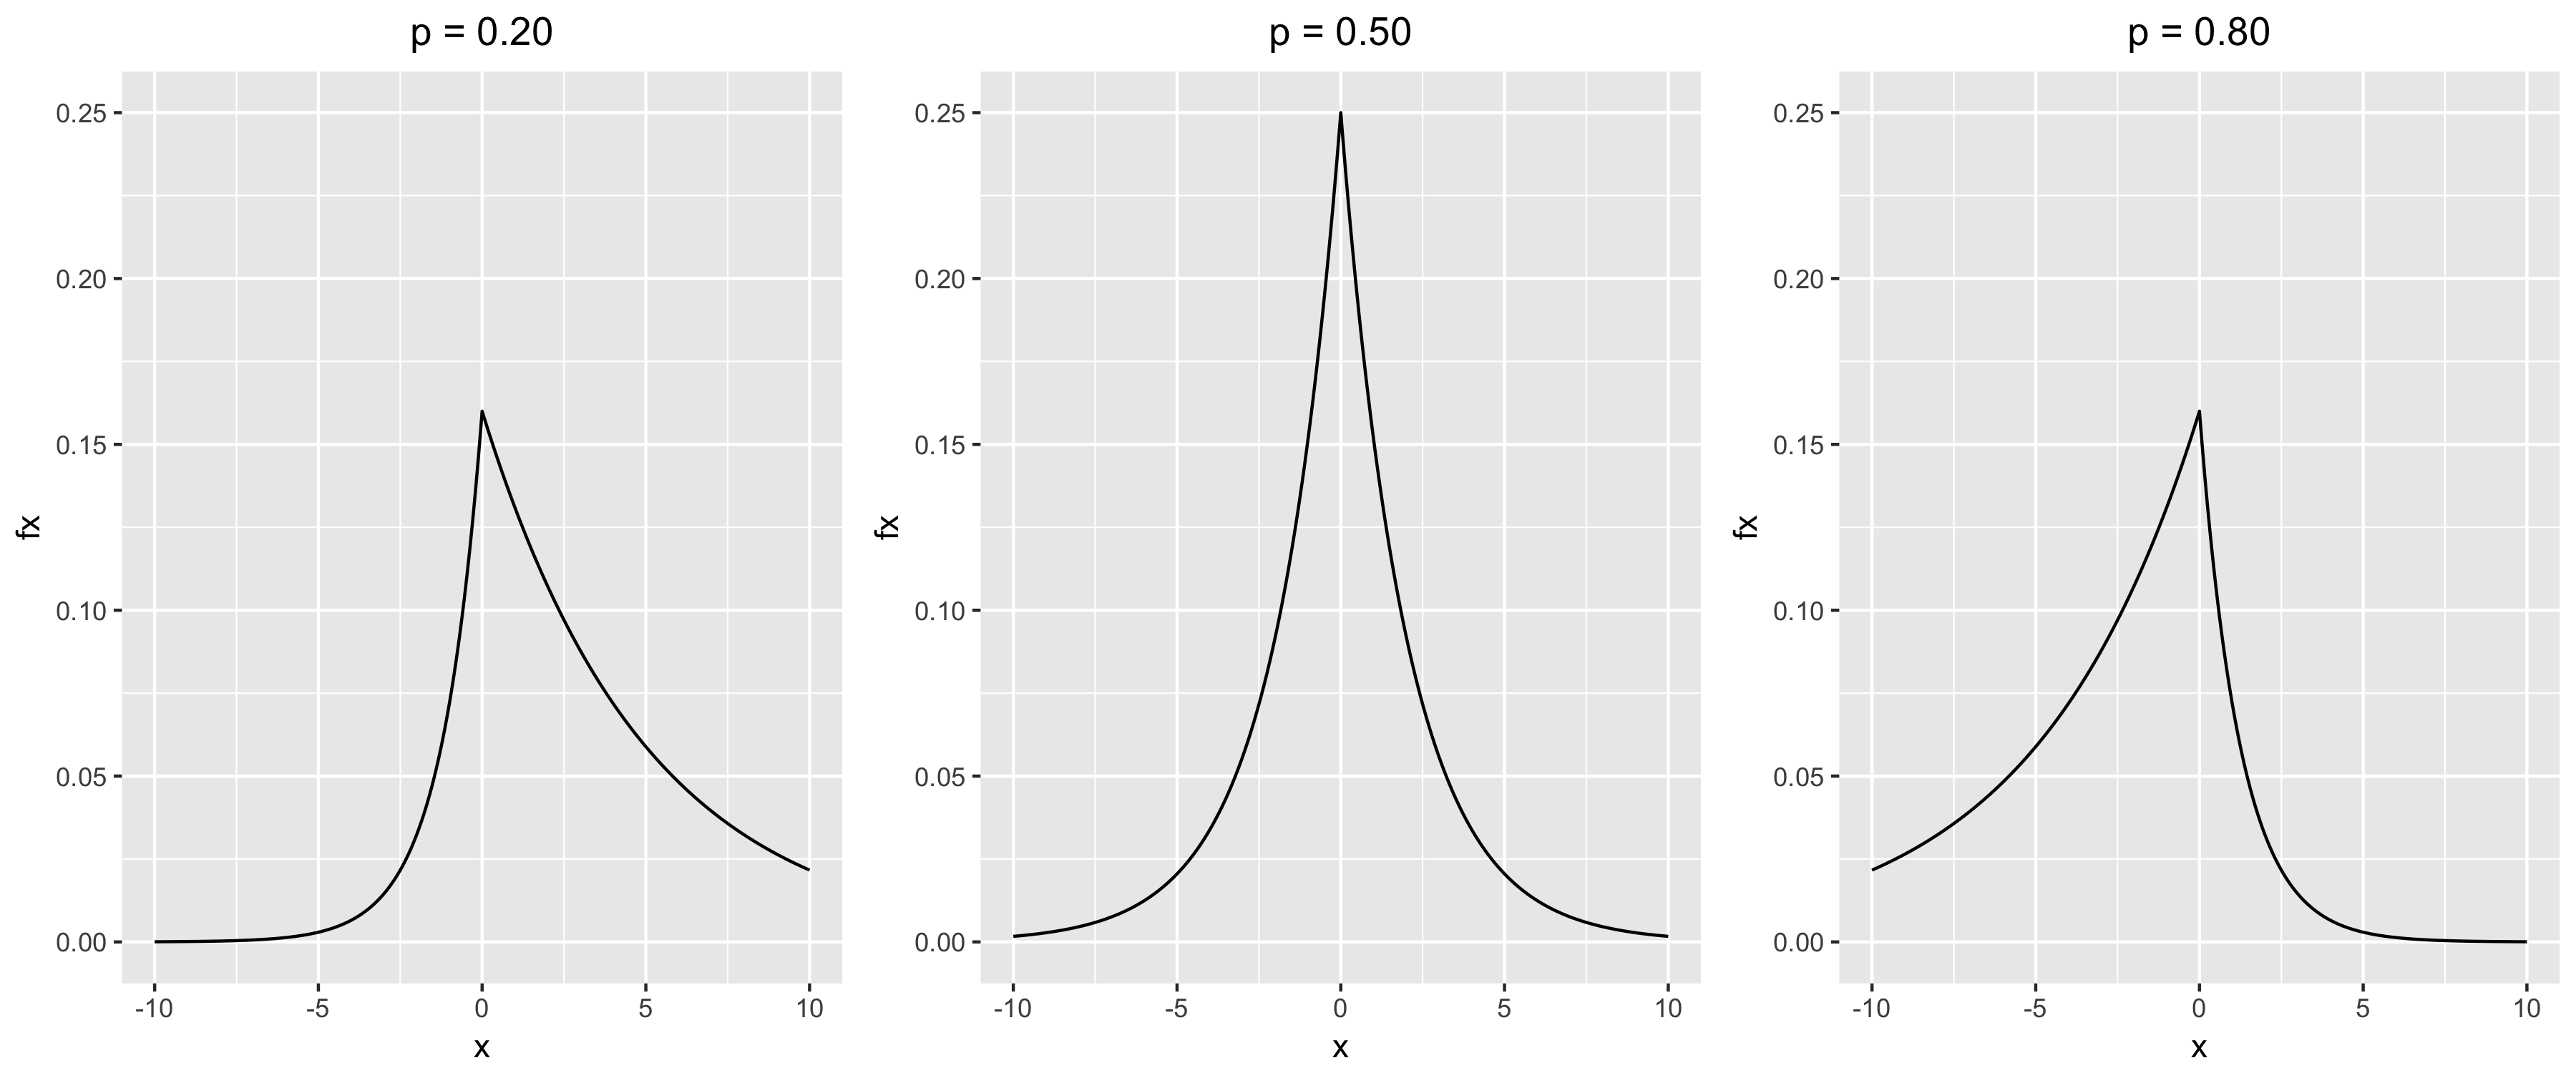
\includegraphics[width=1\textwidth]{Figures/ALD/p_plots.png}
	\label{p_plots}
  \end{figure}
\end{frame}

\begin{frame}{Distribuci\'on asim\'etrica de Laplace}
  \begin{figure}[H]
	\centering
	\caption{Funci\'on de densidad de la distribuci\'on asim\'etrica de Laplace, con $p = 0.25$ y $\sigma$ variable.}
	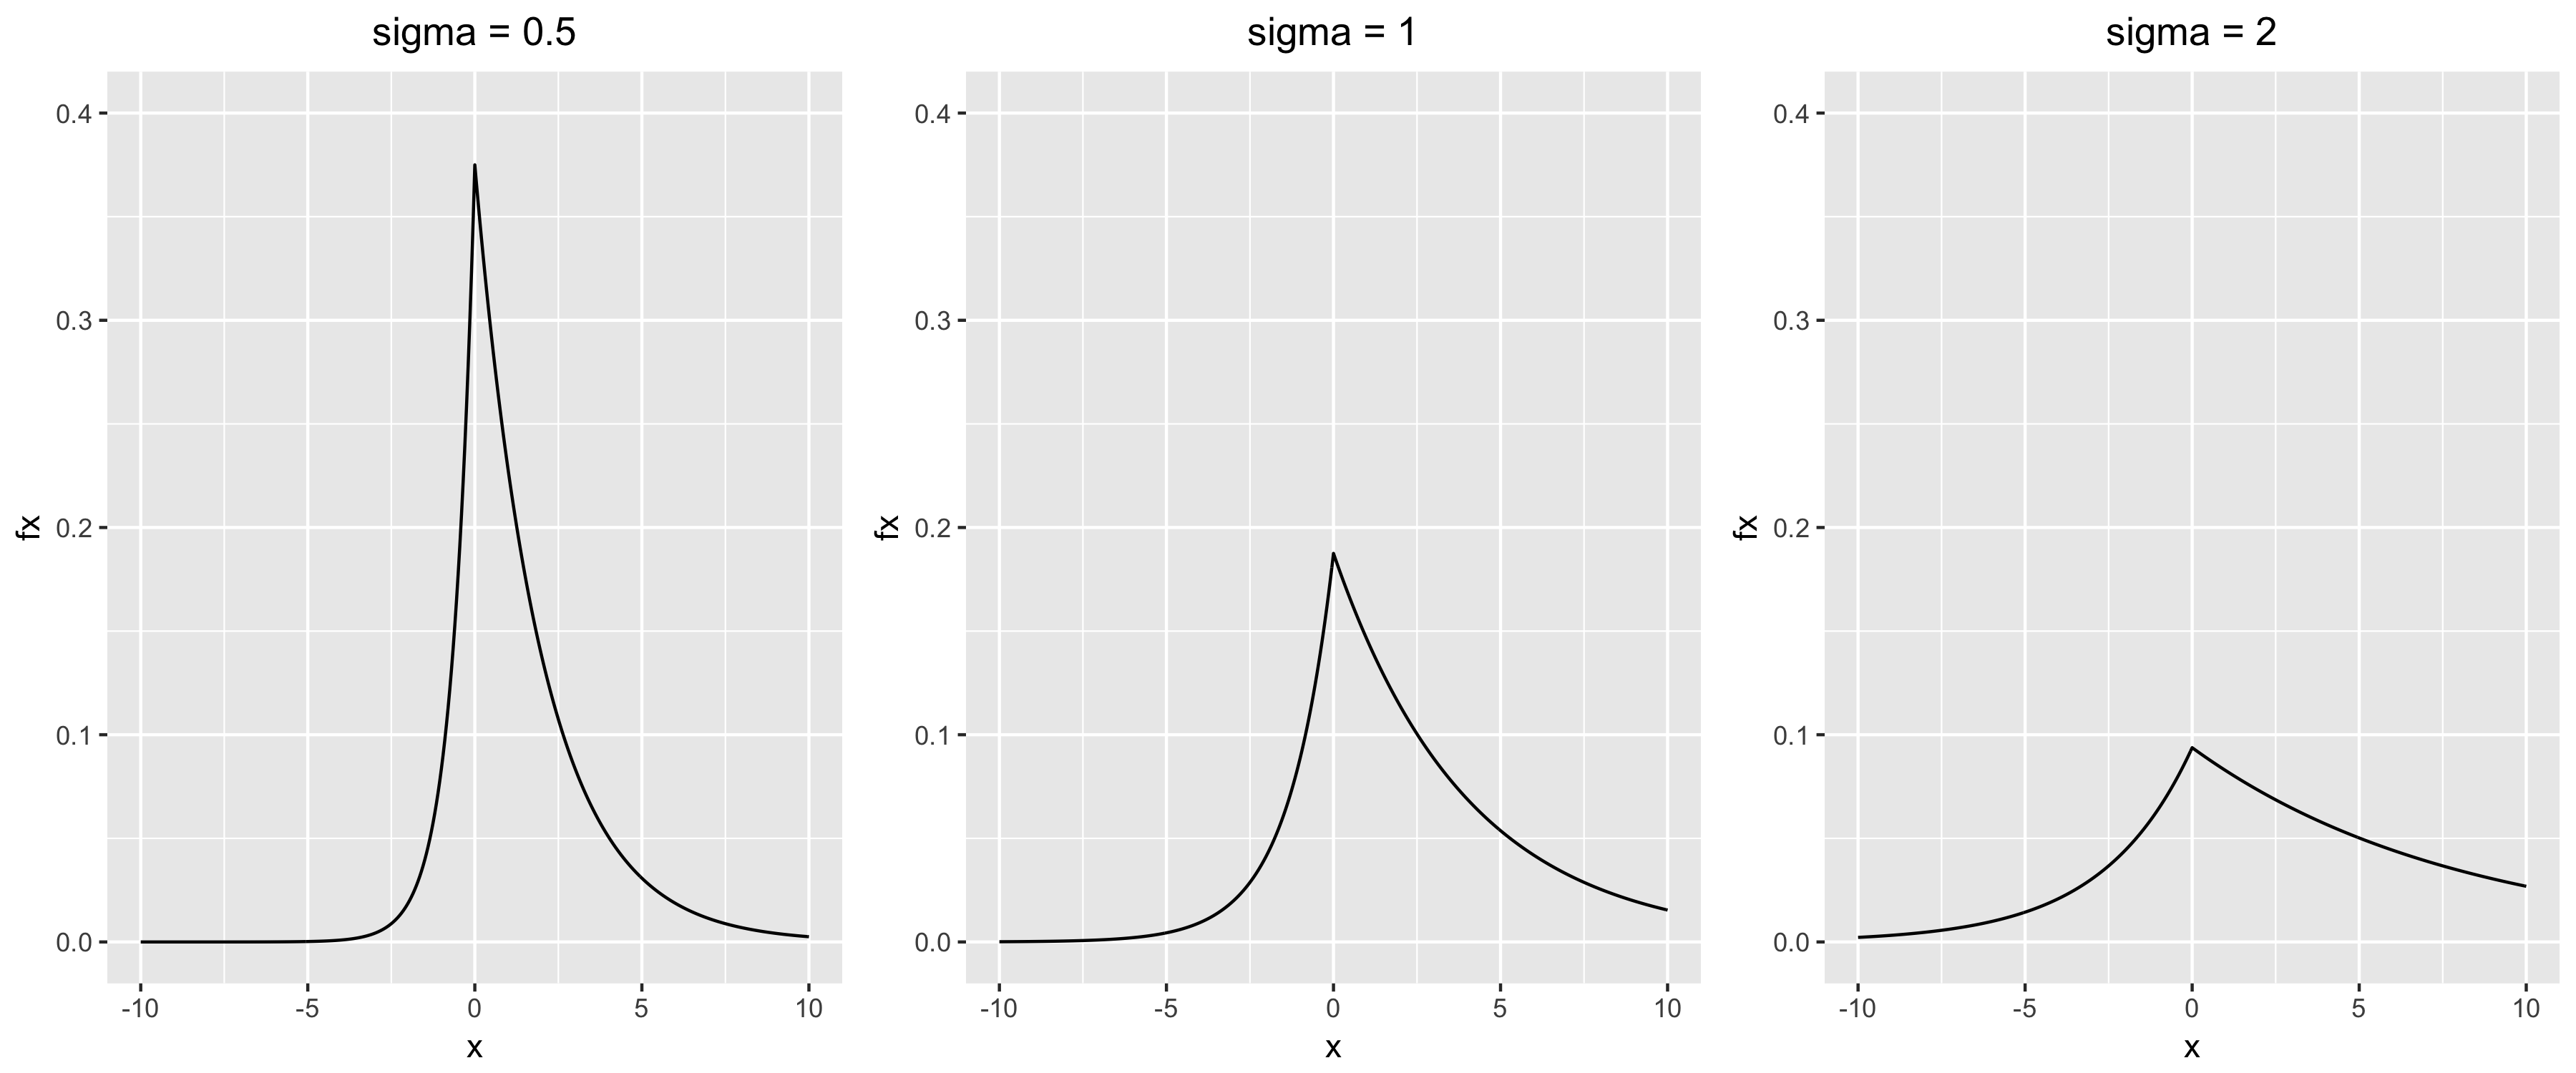
\includegraphics[width=1\textwidth]{Figures/ALD/sigma_plots.png}
	\label{p_plots}
  \end{figure}
\end{frame}


\section{Inferencia no param\'etrica}

\begin{frame}{Estad\'istica no param\'etrica}
\begin{block}{Wasserman (2006)}
    \textit{"La idea b\'asica de la \textbf{inferencia no param\'etrica} es usar los datos para inferir una medida desconocida, haciendo los \textbf{menos supuestos} posibles. Normalmente esto significa usar modelos estad\'isticos de \textbf{dimensi\'on infinita}. De hecho, un mejor nombre para la inferencia no param\'etrica podr\'ia ser \textbf{inferencia de dimensi\'on infinita}."}
\end{block}
\end{frame}

\subsection{Distribuci\'on de $f_p$, mediante procesos Gaussianos}

\begin{frame}{Generalizaci\'on de la relaci\'on lineal}
\begin{itemize}
  \setlength\itemsep{2em}
    \item{Idea: \textbf{generalizar relaci\'on lineal} $f_p(x) = x^T\beta_p$, a \textbf{cualquier posible funci\'on}.} 
    
    \item{Medida de probabilidad para $\bm{\beta_p} \rightarrow$  Medida de probabilidad para $\bm{f_p}$. } 
    
    \item{Como $f_p$ est\'a definida para m\'ultiples valores de $x$, se trata de un conjunto de variables aleatorias que \textbf{depende de variables de entrada}: un \textbf{proceso estoc\'astico}. } 
    
    \item{Para el caso particular de esta tesis, se pensar\'a que  $f_p$ sigue la ley de probabilidad de un \textbf{proceso Gaussiano}.} 
\end{itemize}
\end{frame}

% \begin{frame}{Procesos Gaussianos}
% \begin{block}{Definici\'on}
%     Un \textbf{proceso Gaussiano} es un conjunto de variables aleatorias, tal que todo subconjunto finito de ellas tendr\'a una \textbf{distribuci\'on Gaussiana (Normal) conjunta}.
% \end{block}

% \begin{block}{Caracterizaci\'on}
%     \begin{equation*}
%     \begin{aligned}
%     \bm{f_p} &\sim \bm{\mathcal{GP} (m,k)},\\
%         \textbf{m} &: \text{ funci\'on de \textbf{medias}, y} \\
%         \textbf{k} &: \text{ funci\'on de \textbf{covarianzas}.}
%     \end{aligned}
%     \end{equation*}
%     \end{block}
% \end{frame}

% \begin{frame}{Procesos Gaussianos}

% \begin{equation*}
% \begin{aligned}
%     M(X) &=     
%     \left[
%         \begin{array}{c}
%         m(x_1)  \\
%         \vdots \\
%         m(x_m)
%         \end{array}
%     \right]
% \end{aligned}
% \end{equation*}

% \begin{equation*}
% \begin{aligned}
%     K(X,X') &=     
%     \left[
%         \begin{array}{ccc}
%         k(x_1,x_1') & ... & k(x_1,x_r')  \\
%         \vdots & \ddots & \vdots \\
%         k(x_m,x_1') & ... & k(x_m,x_r')
%         \end{array}
%     \right]
% \end{aligned}
% \end{equation*}

% \\~\\

% \begin{equation*}
% \begin{aligned}
%     \implies \bm{f_p(X)} \sim  \bm{\mathcal{N}(M(X), K(X,X))}
% \end{aligned}
% \end{equation*}
% \end{frame}


% \begin{frame}{Predicci\'on de los procesos Gaussianos}

% Sean 
% \begin{equation*}
%     \left[
%         \begin{array}{c}
%         f_p(X)  \\
%         f_p(X_*) 
%         \end{array}
%     \right]  
%     \sim \mathcal{N}  
%     \left(
%         \left[
%             \begin{array}{c} 
%             M(X) \\ 
%             M(X_*) 
%             \end{array}
%         \right],
%         \left[
%             \begin{array}{cc}
%             K(X,X) & K(X,X_*)  \\
%             K(X_*,X) & K(X_*,X_*) 
%             \end{array}
%         \right]
%     \right).
% \end{equation*}

% Bajo el supuesto de que ya se conocen las \textbf{observaciones de} $\bm{f_p(X)}$, entonces, por las propiedades de la \textbf{distribuci\'on Normal condicional},

% \begin{equation*}
%     f_p(X_*)|f_p(X) 
%     \sim \mathcal{N}
%     (\bar{M}(X,X_*),\bar{K}(X,X_*)),
% \end{equation*}
% con
% \begin{equation*}
% \begin{aligned}
%     \bar{M}(X,X_*) &= M(X_*) + K(X_*,X)K(X,X)^{-1}(f_p(X) - M(X)), \\
%     \bar{K}(X,X_*) &= K(X_*,X_*) - K(X_*,X)K(X,X)^{-1}K(X,X_*).
% \end{aligned}
% \end{equation*}

% \end{frame}

\subsection{Distribuci\'on de $\varepsilon_p$, mediante procesos de Dirichlet}

\begin{frame}{Error no param\'etrico}
    \begin{block}{Intuici\'on de los procesos de Dirichlet}
        Las realizaciones $\varepsilon_1,...,\varepsilon_n$ provienen de una \textbf{distribuci\'on} $\bm G$, la cual es \textbf{desconocida} para el modelador. 
        \\~\\
        Para reflejar su \textbf{incertidumbre}, le asigna una \textbf{ley de probabilidad} a los posibles valores de $G$, particularmente la de un \textbf{proceso de Dirichlet}.
        \\~\\
        Es decir, \textbf{la realizaci\'on de un proceso de Dirichlet es una distribuci\'on de probabilidad}.
    \end{block}
\end{frame}

% \begin{frame}{Procesos de Dirichlet}
%     \begin{block}{Definici\'on}
%         Sean $\bm{G}$ y $\bm{H}$ \textbf{dos distribuciones} cuyo soporte es el conjunto $\Theta$ y sea $\alpha \in \mathbb{R}_+$. Si se toma una \textbf{partici\'on finita cualquiera} $(A_1,\ldots,A_r)$ del conjunto $\Theta$, se entender\'a que $\bm{G(A_i)}$  es la \textbf{ probabilidad de que una realizaci\'on de} $\bm{G}$ \textbf{pertenezca al conjunto} $\bm{A_i}$.
%         \\~\\
%         Se dice que $G$ sigue la distribuci\'on de un \textbf{proceso de Dirichlet} $\bm{(G \sim DP(\alpha,H))}$, con \textbf{distribuci\'on media} $\bm{H}$ y \textbf{par\'ametro de concentraci\'on} $\bm{\alpha}$, si
%         \begin{equation*}
%             \bm{(G(A_1),\ldots,G(A_r))} \sim \bm{ Dir(\alpha H(A_1),\ldots,\alpha H(A_r))}, 
%         \end{equation*}
%         para cualquier partici\'on finita $(A_1,\ldots,A_r)$ del conjunto $\Theta$.
%     \end{block}
% \end{frame}

% \begin{frame}{Procesos de Dirichlet}
%     Sean $\phi_1,...,\phi_n$ realizaciones de la distribuci\'on $G$. Si $\phi_{n+1}$ sigue la misma ley de probabilidad, se tiene entonces que 
%     \begin{equation*}
%     \phi_{n+1}|\phi_1,...,\phi_n \sim 
%     \left(\frac{\bm{\alpha}}{\alpha + n}\right)\bm{H}(\phi_{n+1}) + 
%     \left(\frac{\bm{n}}{\alpha + n}\right)\frac{\sum_{i=1}^n \delta_i(\phi_{n+1})}{n}.
%     \end{equation*}
%     La distribuci\'on predictiva tiene \textbf{puntos de masa} localizados en $\phi_1,...,\phi_n$, lo que significa que la \textbf{probabilidad} de que $\phi_{n+1}$ tome esos valores en espec\'ifico es \textbf{mayor a 0}. 
    
%     Esa es la intuici\'on por la que $\bm{G}$ \textbf{es una distribuci\'on discreta casi seguramente}.
% \end{frame}

% \begin{frame}{Proceso estoc\'astico de rompimiento de un palo}
%     Dado que $G \sim DP(\alpha,H)$  es una distribuci\'on discreta casi seguramente, se puede expresar como una suma de centros de masa de la siguiente manera:
%     \begin{equation*}
%     \begin{aligned}
%     G(\phi) &= \sum_{k=1}^\infty \pi_k \delta_{\phi_k^*}(\phi),\\
%       \phi_k^* &\sim H,
%     \end{aligned}
%     \end{equation*}
%     siendo $\pi_k$ la probabilidad de ocurrencia de $\phi_k^*$.
%     \begin{equation*}
%   \begin{aligned}
%       \beta_k &\sim Beta(1,\alpha),\\
%       \pi_1 &= \beta_1, \\
%       \pi_k &= \beta_k \prod_{i=1}^{k-1}(1 - \beta_i) 
%       \text{, para k $\geq$ 2.}
%     \end{aligned}
%     \end{equation*}
%     Se denomina $\pi \sim GEM(\alpha)$, en honor a Griffiths, Engen y McCloskey.
% \end{frame}

% \begin{frame}{Modelo de mezclas infinitas de Dirichlet para la distribuci\'on asim\'etrica de Laplace}
%     \begin{equation*}
%     \begin{aligned}
%       {\varepsilon_p}_i | z_i, \sigma_k^* &\sim \mathcal{AL}_p({\varepsilon_p}_i | \sigma_{z_i}), \\
%       z_i | \pi &\sim \mathrm{Mult}_{\infty}(\pi)\footnotemark, \\
%       \pi | \alpha &\sim GEM(\alpha), \\
%       \sigma_k^* | H &\sim H.
%     \end{aligned}
%     \end{equation*}
%     \footnotetext{Se usar\'a la notaci\'on $\mathrm{Mult}_{\infty}$ para denotar al l\'imite de la distribuci\'on Multinomial, cuando el n\'umero de posibles categor\'ias tiende a infinito.}
% \end{frame}

\section{Modelo GPDP}

\begin{frame}{Descripci\'on Modelo GPDP}
    \begin{equation*}
    \begin{aligned}
        y_i| f_p(x_i), z_i, \sigma_k^* &\sim \mathcal{AL}_p({\varepsilon_p}_i = y_i - f_p(x_i) | \sigma_{z_i}), \\
        f_p|m, k, \lambda &\sim \mathcal{GP}(m,k(\lambda)|\lambda), \\
        \lambda &\sim GI(c_\lambda,d_\lambda), \\
        z_i | \pi &\sim \mathrm{Mult}_{\infty}(\pi), \\
        \pi | \alpha &\sim GEM(\alpha), \\
        \sigma_k^* | c_{DP}, d_{DP} &\sim GI(\sigma_k|c_{DP}, d_{DP}),\\
        k(x_i, x_j | \lambda) &= \lambda \text{ } exp\{-\norm{x_i - x_j}_2\}.
    \end{aligned}
    \end{equation*}
\end{frame}

\begin{frame}{Paquete \textit{GPDPQuantReg} en R}
    \begin{Large} Github \faGithub \space: \textbf{opardo/GPDPQuantReg} \end{Large}
    \\~\\
    3 funciones p\'ublicas:
    \begin{itemize}
        \item \textbf{GPDPQuantReg}: ajusta el modelo con los datos que recibe
        \item \textbf{predict}: realiza predicci\'on para un conjunto de covariables
        \item \textbf{diagnose}: diagn\'ostico de las cadenas de Markov del simulador de Gibbs \footnote{Algoritmo MCMC, para realizar inferencia Bayesiana.}
    \end{itemize}{}
\end{frame}

\section{Aplicaciones}

\begin{frame}{Comparaci\'on de modelos}
    \begin{table}[H]
    \centering
    \begin{tabular}{ccc}
    \hline
     & \textbf{Modelo Tradicional} & \textbf{Modelo GPDP} \\ 
    \hline
    \textbf{Par\'ametro de regresi\'on} & A la media & Sobre cuantiles \\ 
    \textbf{Relaci\'on entre $\bm x$ y $ \bm y$} & Lineal & No lineal \\ 
    \textbf{Tipo de error} & Param\'etrico & No param\'etrico \\ 
    \hline
    \end{tabular}
\end{table}
\end{frame}

\begin{frame}{Simulaci\'on de datos}
\begin{block}{}
    \begin{equation*}
    \begin{aligned}
        y &= g(x) + \omega,\\
        g(x) &: \text{ funci\'on determinista,} \\
        \omega &: \text{ variable aleatoria}
    \end{aligned}
    \end{equation*}
    \\~\\
    \begin{equation*}
        \implies \bm{f_p(x) = g(x) + q_p(\omega)}
    \end{equation*}
\end{block}
\end{frame}

\begin{frame}{Supuestos tradicionales de regresi\'on}
    \begin{figure}[H]
        	\centering
        	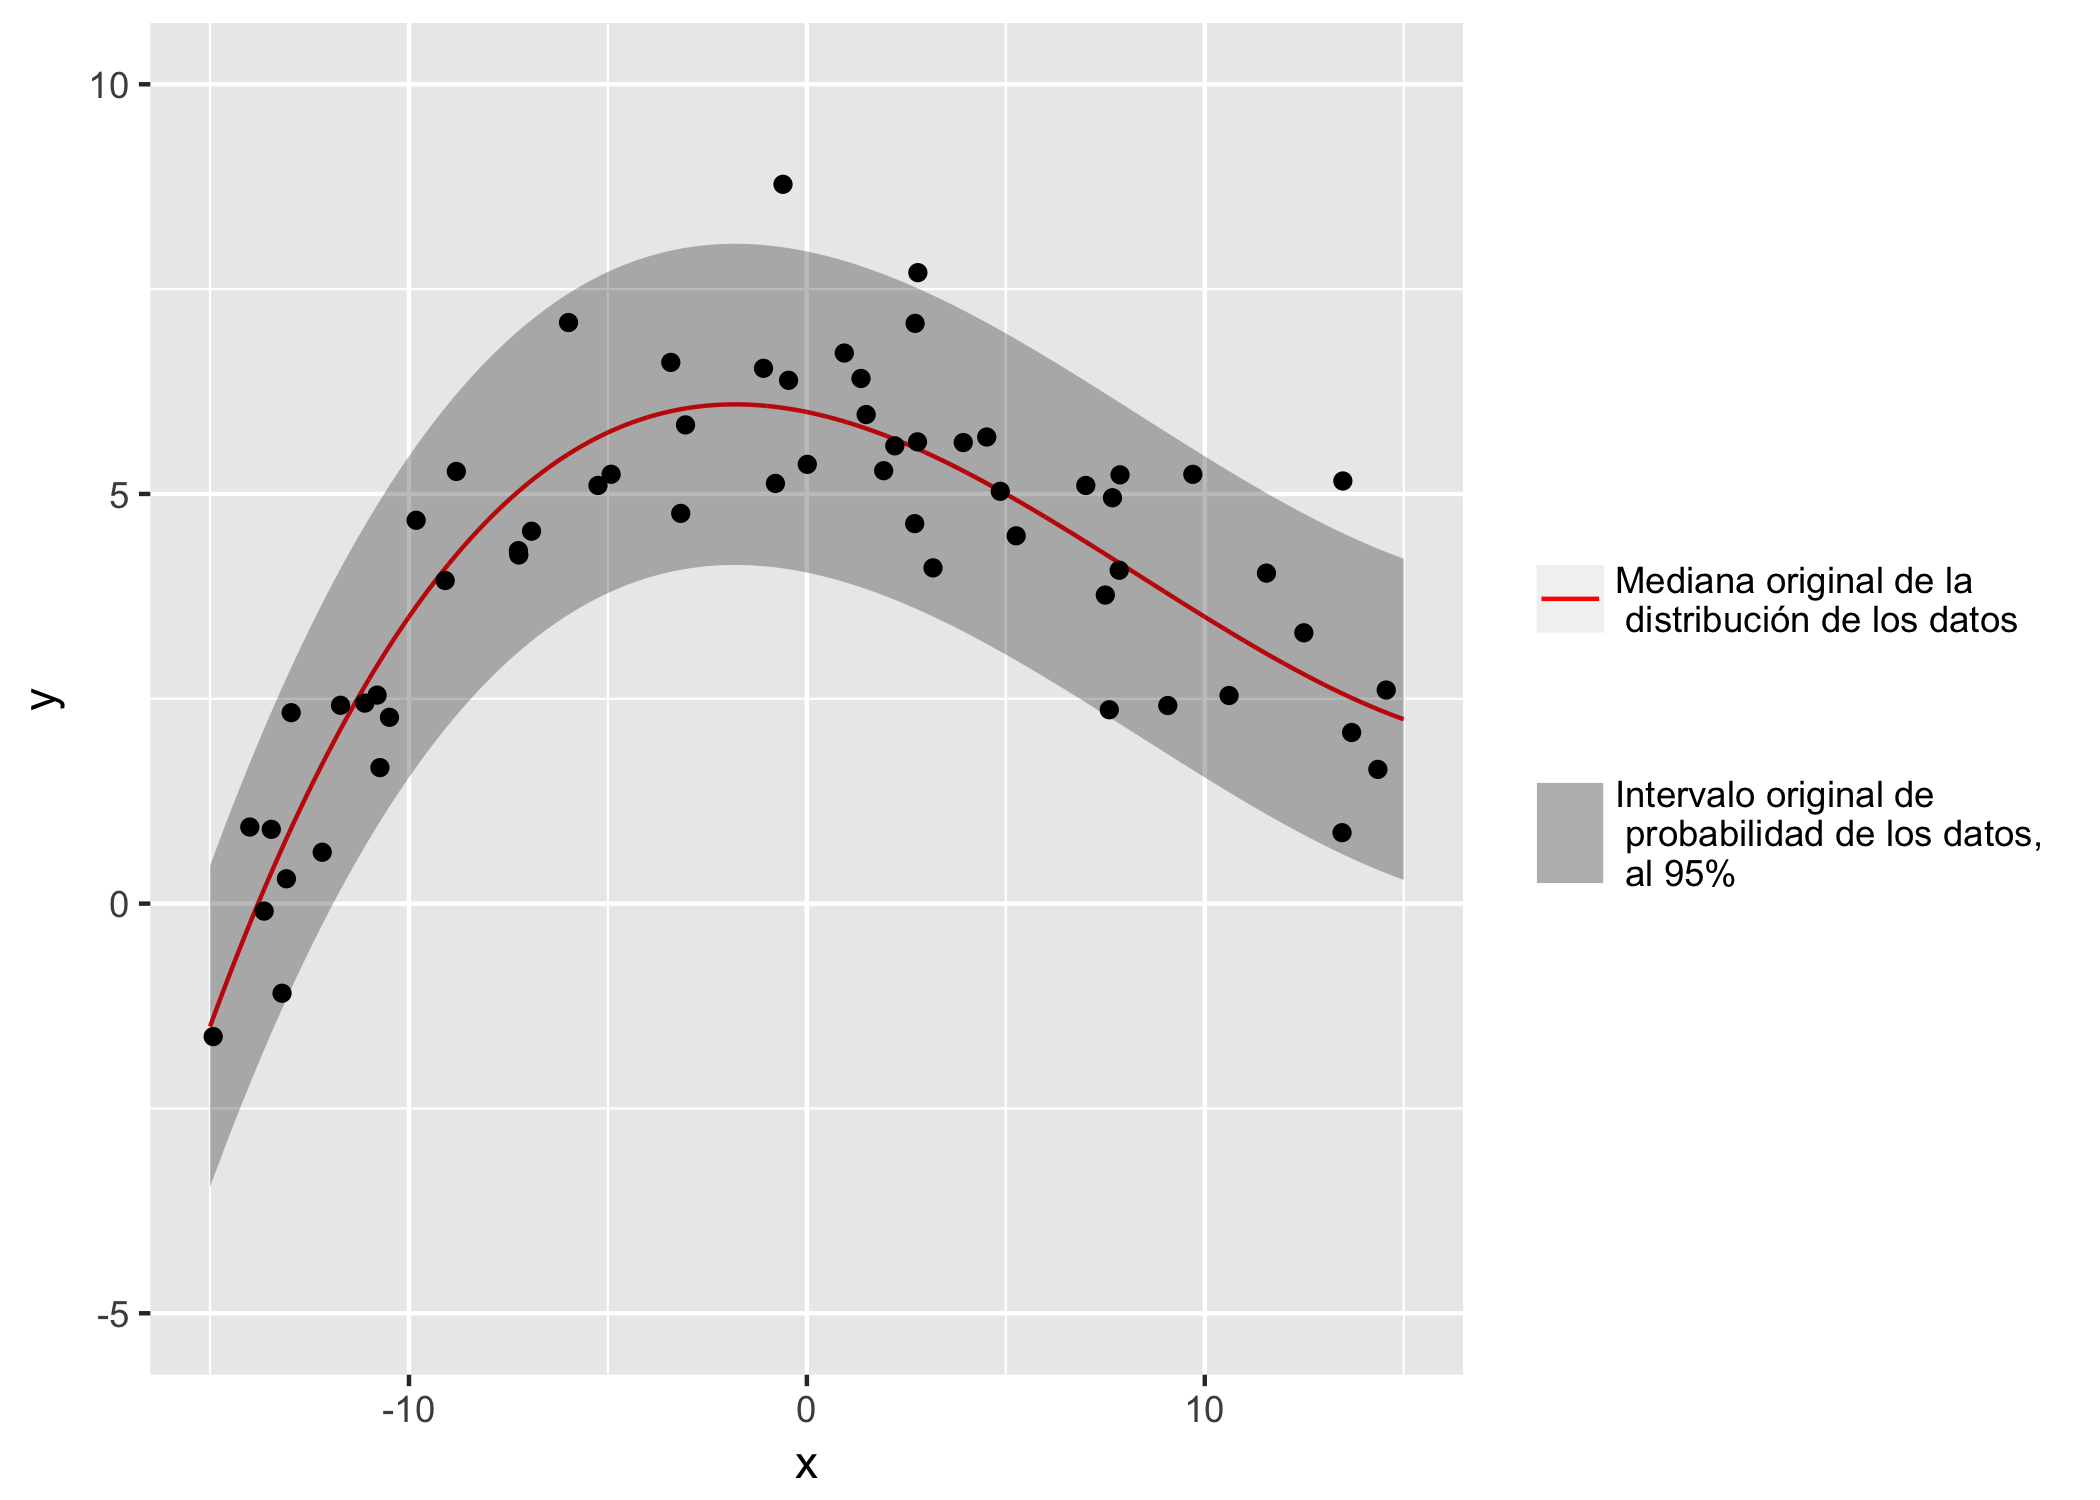
\includegraphics[width=0.7\textwidth]{Figures/Simulation/classic/sample.png}
        	\label{sample_classic}
    \end{figure}
    \begin{equation*}
    \begin{aligned}
        g(x) &= \frac{1}{1000}x^3 - \frac{1}{40}x^2 - \frac{1}{10}x + 6,\\
        \omega &\sim \mathcal{N}(0,1)
    \end{aligned}
    \end{equation*}
\end{frame}

\begin{frame}{Supuestos tradicionales de regresi\'on}
    \begin{figure}[H]
        \centering
        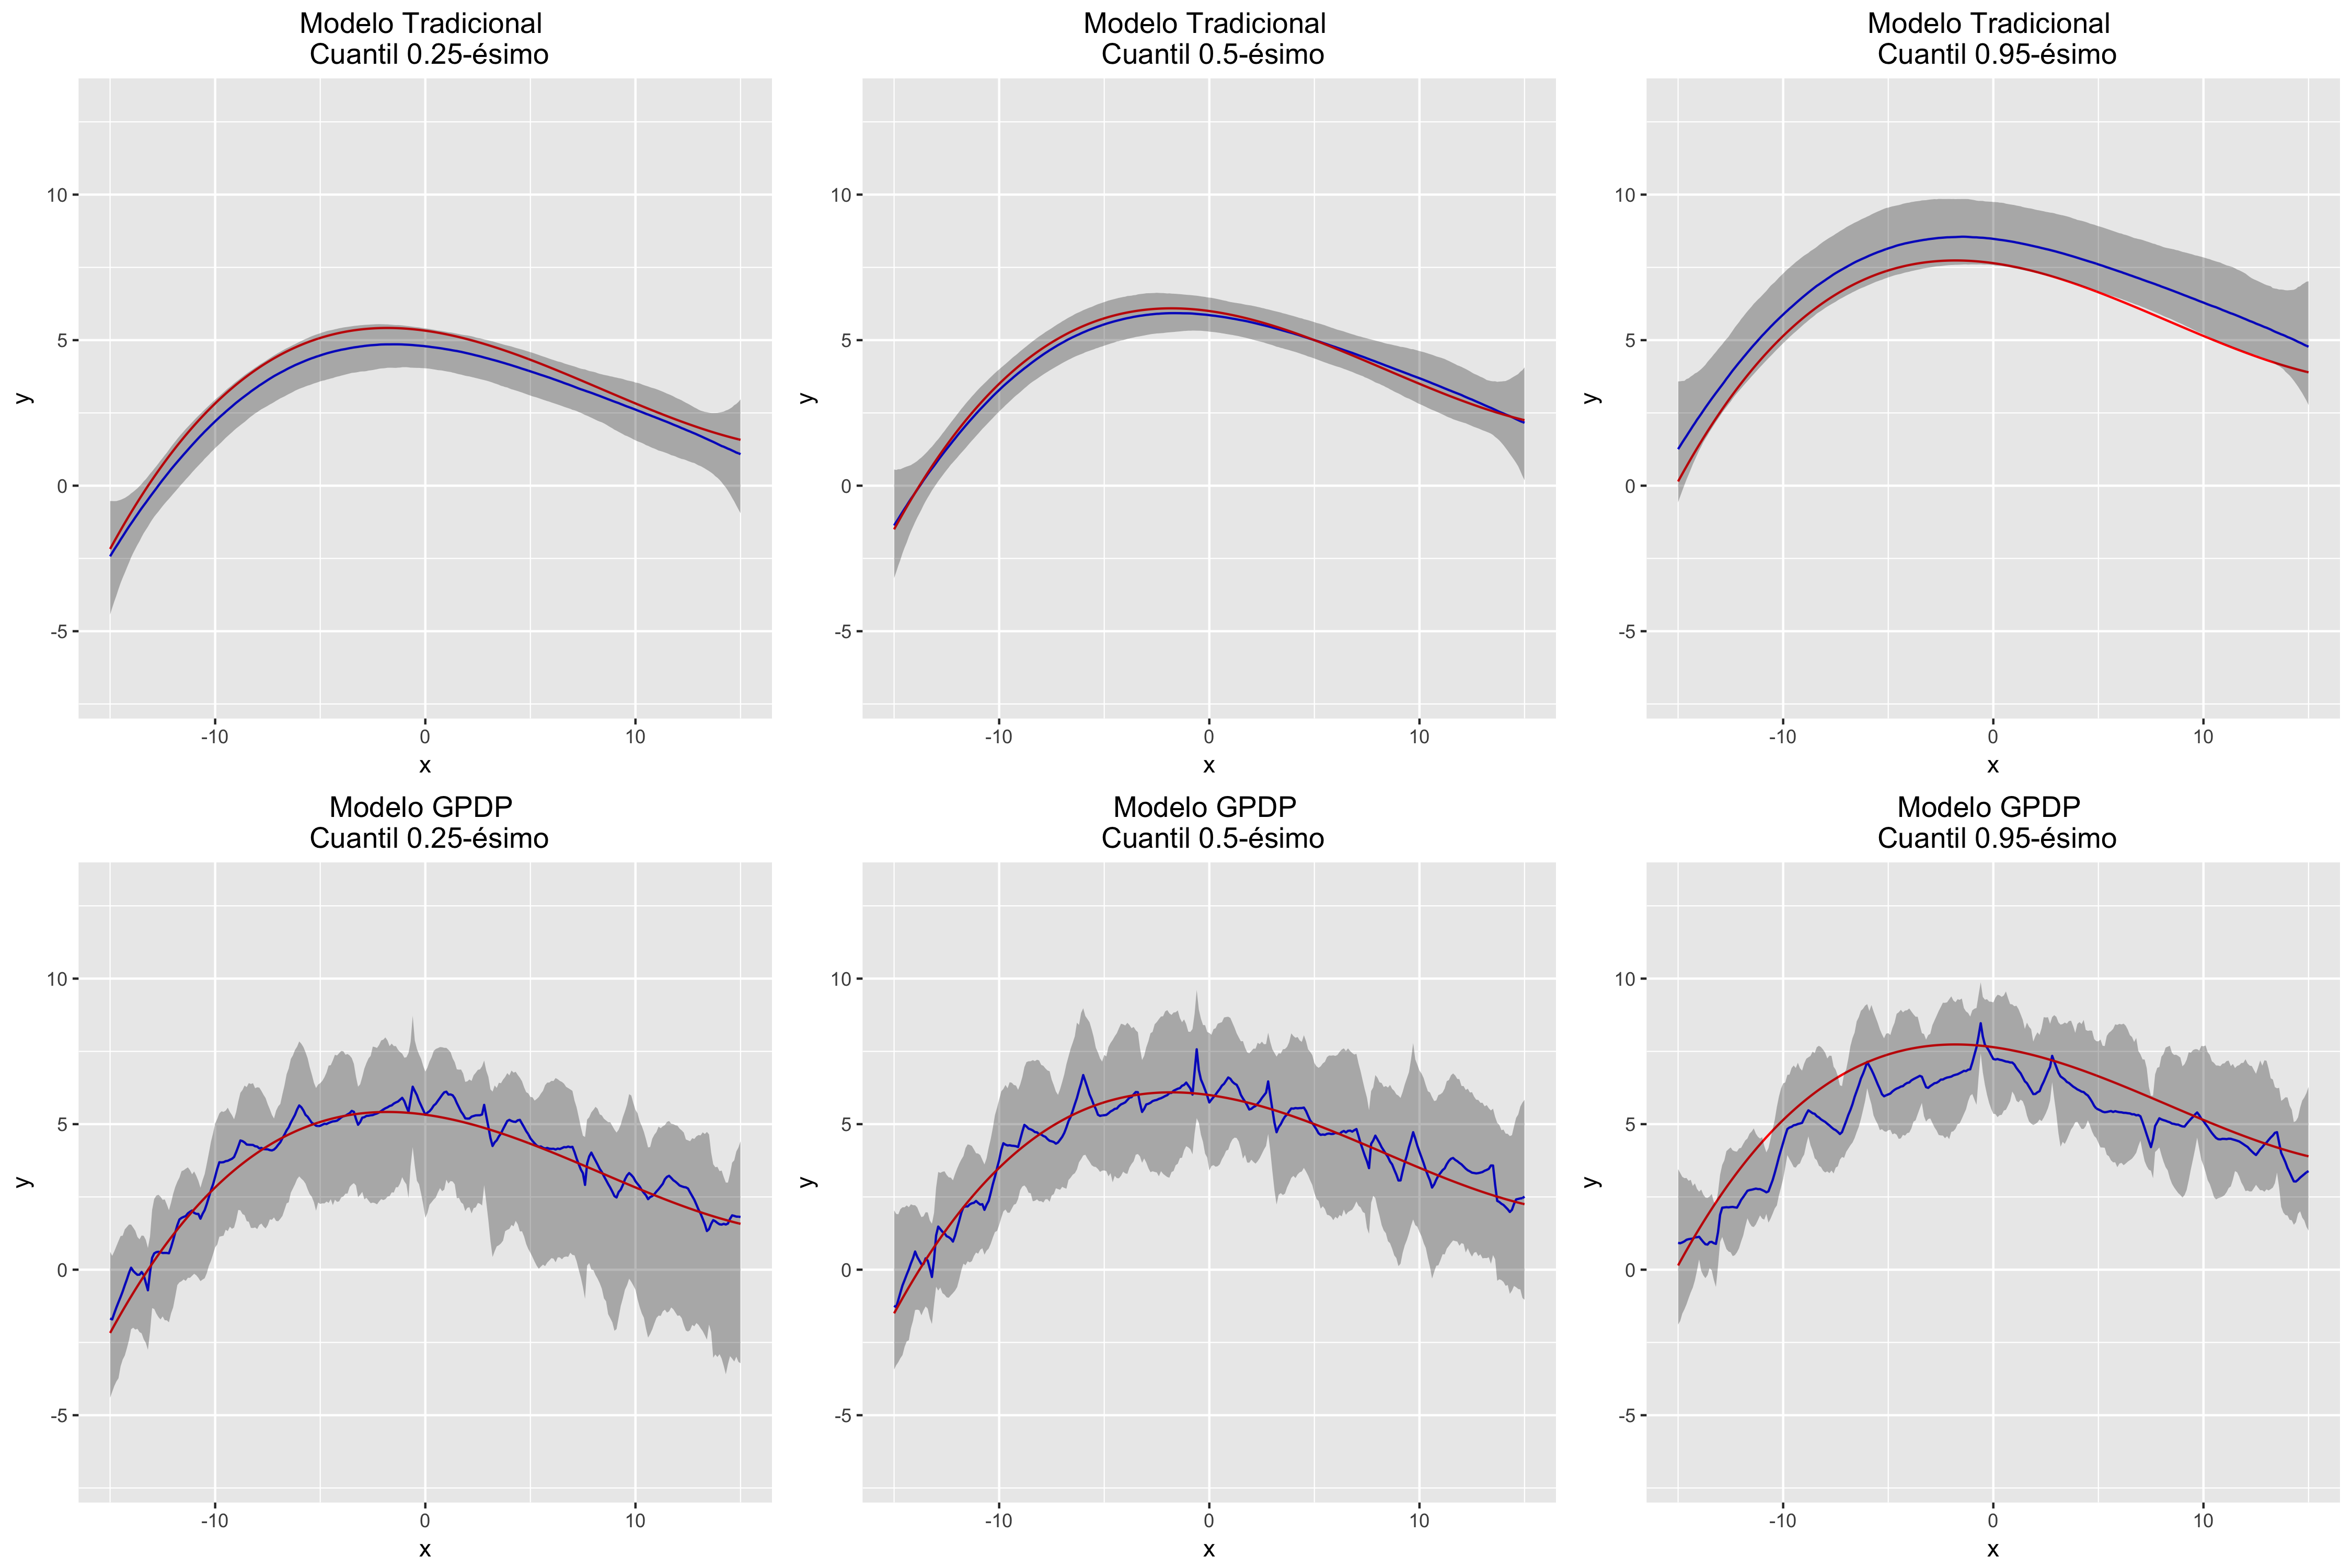
\includegraphics[width=0.8\textwidth]{Figures/Simulation/classic/presentation.png}
        \captionsetup{singlelinecheck=off,font=footnotesize}
        \caption*{Nota: La l\'inea roja representa el valor real de cada cuantil, la l\'inea azul representa la mediana de la distribuci\'on posterior predictiva y el \'area gris su intervalo de probabilidad al 95\%.}
    \end{figure}
\end{frame}

\begin{frame}{Supuestos tradicionales de regresi\'on}

\begin{scriptsize}

\begin{table}[H]
    \centering
    \caption{Error cuadr\'atico medio entre mediana predictiva y cuantil real}
    \begin{tabular}{ccc}
    \hline
    Cuantil & Modelo Tradicional & Modelo GPDP \\ 
    \hline
    0.95 & 0.84 & 0.83 \\ 
    0.50 & 0.02 & 0.19 \\ 
    0.25 & 0.23 & 0.16 \\ 
    \hline
    \end{tabular}
\end{table}
\begin{table}[H]
    \centering
    \caption{Correlaci\'on al cuadrado entre mediana predictiva y cuantil real} 
    \begin{tabular}{ccc}
    \hline
    Cuantil & Modelo Tradicional & Modelo GPDP \\ 
    \hline
    0.95 & 0.99 & 0.91 \\ 
    0.50 & 0.99 & 0.94 \\ 
    0.25 & 0.99 & 0.96 \\ 
    \hline
    \end{tabular}
\end{table}

\begin{table}[H]
    \centering
    \caption{Porcentaje de valores reales dentro del intervalo de confianza al 95$\%$} 
    \begin{tabular}{ccc}
    \hline
    Cuantil & Modelo Tradicional & Modelo GPDP \\ 
    \hline
    0.95 & 68\% & 96\% \\ 
    0.50 & 100\% & 100\% \\ 
    0.25 & 100\% & 100\% \\ 
    \hline
    \end{tabular}
\end{table}

\end{scriptsize}
\end{frame}

\begin{frame}{Error aleatorio de colas pesadas}
    \begin{figure}[H]
        	\centering
        	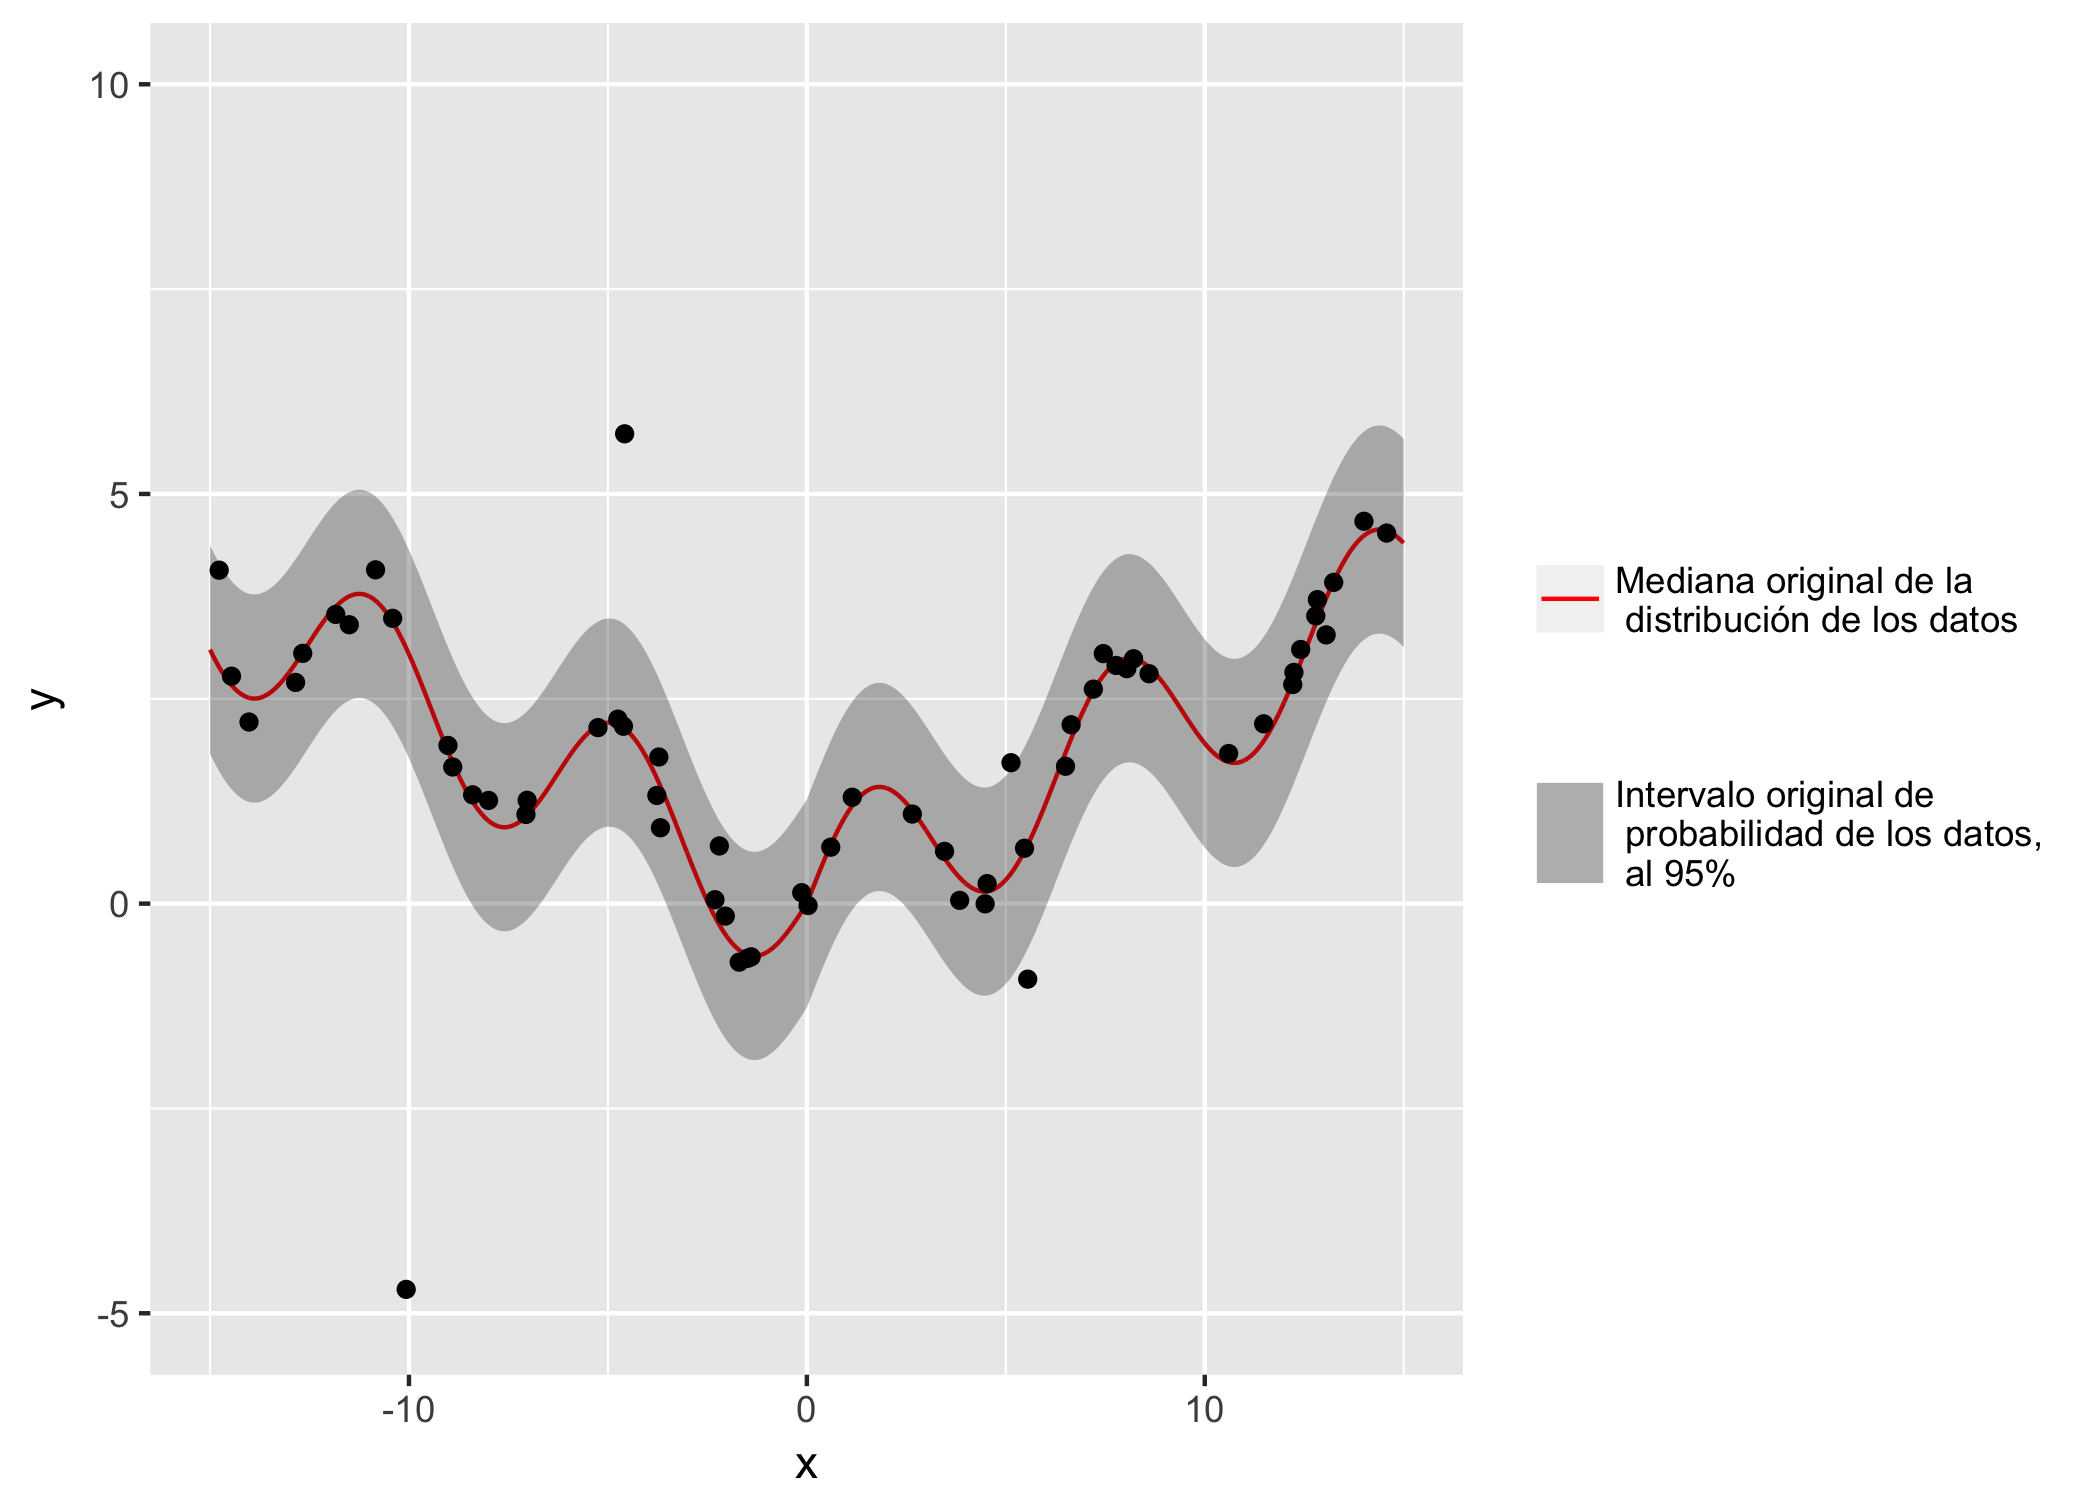
\includegraphics[width=0.7\textwidth]{Figures/Simulation/heavy_tails/sample.png}
        	\label{sample_classic}
    \end{figure}
    \begin{equation*}
    \begin{aligned}
        g(x) &= \frac{1}{4}|x| + sen(x),\\
        \omega &\sim Cauchy(0,0.1)
    \end{aligned}
    \end{equation*}
\end{frame}

\begin{frame}{Error aleatorio de colas pesadas}
    \begin{figure}[H]
        \centering
        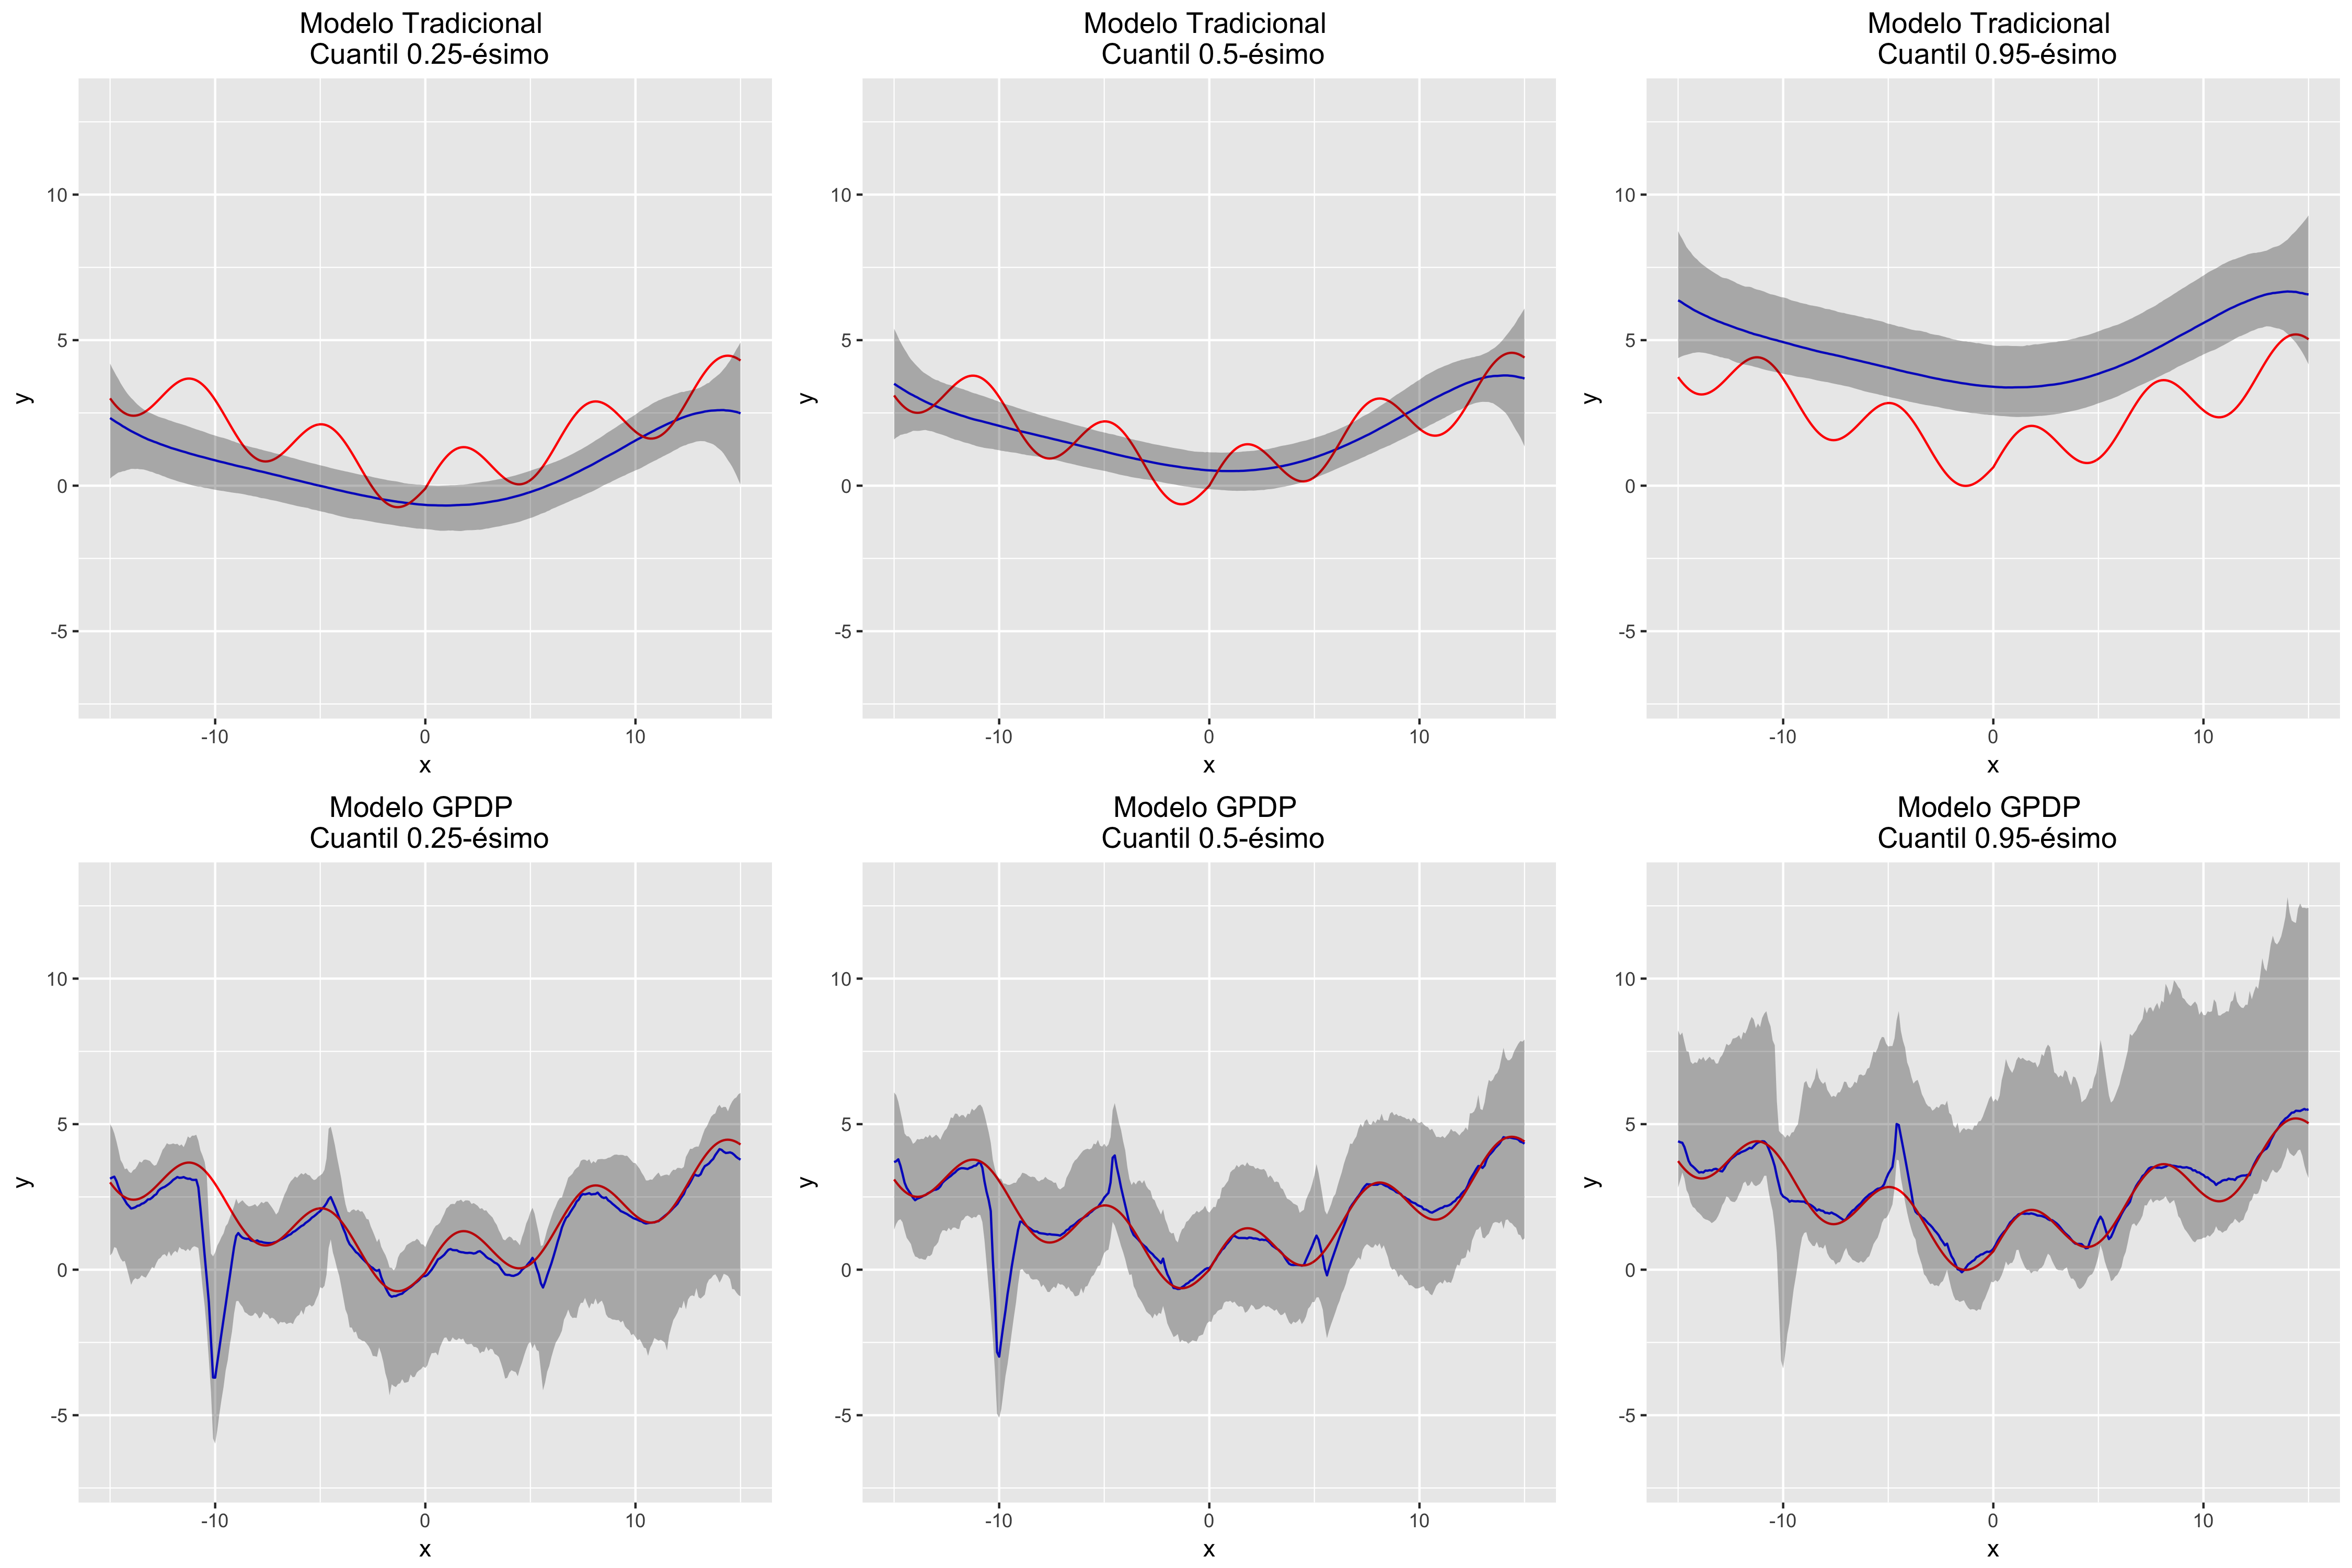
\includegraphics[width=0.8\textwidth]{Figures/Simulation/heavy_tails/presentation.png}
        \captionsetup{singlelinecheck=off,font=footnotesize}
        \caption*{Nota: La l\'inea roja representa el valor real de cada cuantil, la l\'inea azul representa la mediana de la distribuci\'on posterior predictiva y el \'area gris su intervalo de probabilidad al 95\%.}
    \end{figure}
\end{frame}

\begin{frame}{Error aleatorio de colas pesadas}

\begin{scriptsize}

\begin{table}[H]
    \centering
    \caption{Error cuadr\'atico medio entre mediana predictiva y cuantil real}
    \begin{tabular}{ccc}
    \hline
    Cuantil & Modelo Tradicional & Modelo GPDP \\ 
    \hline
    0.95 & 5.42 & 0.18 \\ 
    0.50 & 0.61 & 0.75 \\ 
    0.25 & 1.89 & 1.12 \\ 
    \hline
    \end{tabular}
\end{table}
\begin{table}[H]
    \centering
    \caption{Correlaci\'on al cuadrado entre mediana predictiva y cuantil real} 
    \begin{tabular}{ccc}
    \hline
    Cuantil & Modelo Tradicional & Modelo GPDP \\ 
    \hline
    0.95 & 0.64 & 0.91 \\ 
    0.50 & 0.64 & 0.64 \\ 
    0.25 & 0.64 & 0.57 \\ 
    \hline
    \end{tabular}
\end{table}

\begin{table}[H]
    \centering
    \caption{Porcentaje de valores reales dentro del intervalo de confianza al 95$\%$} 
    \begin{tabular}{ccc}
    \hline
    Cuantil & Modelo Tradicional & Modelo GPDP \\ 
    \hline
    0.95 & 9\% & 98\% \\ 
    0.50 & 57\% & 100\% \\ 
    0.25 & 41\% & 96\% \\ 
    \hline
    \end{tabular}
\end{table}

\end{scriptsize}
\end{frame}

\begin{frame}{Error aleatorio asim\'etrico}
    \begin{figure}[H]
        	\centering
        	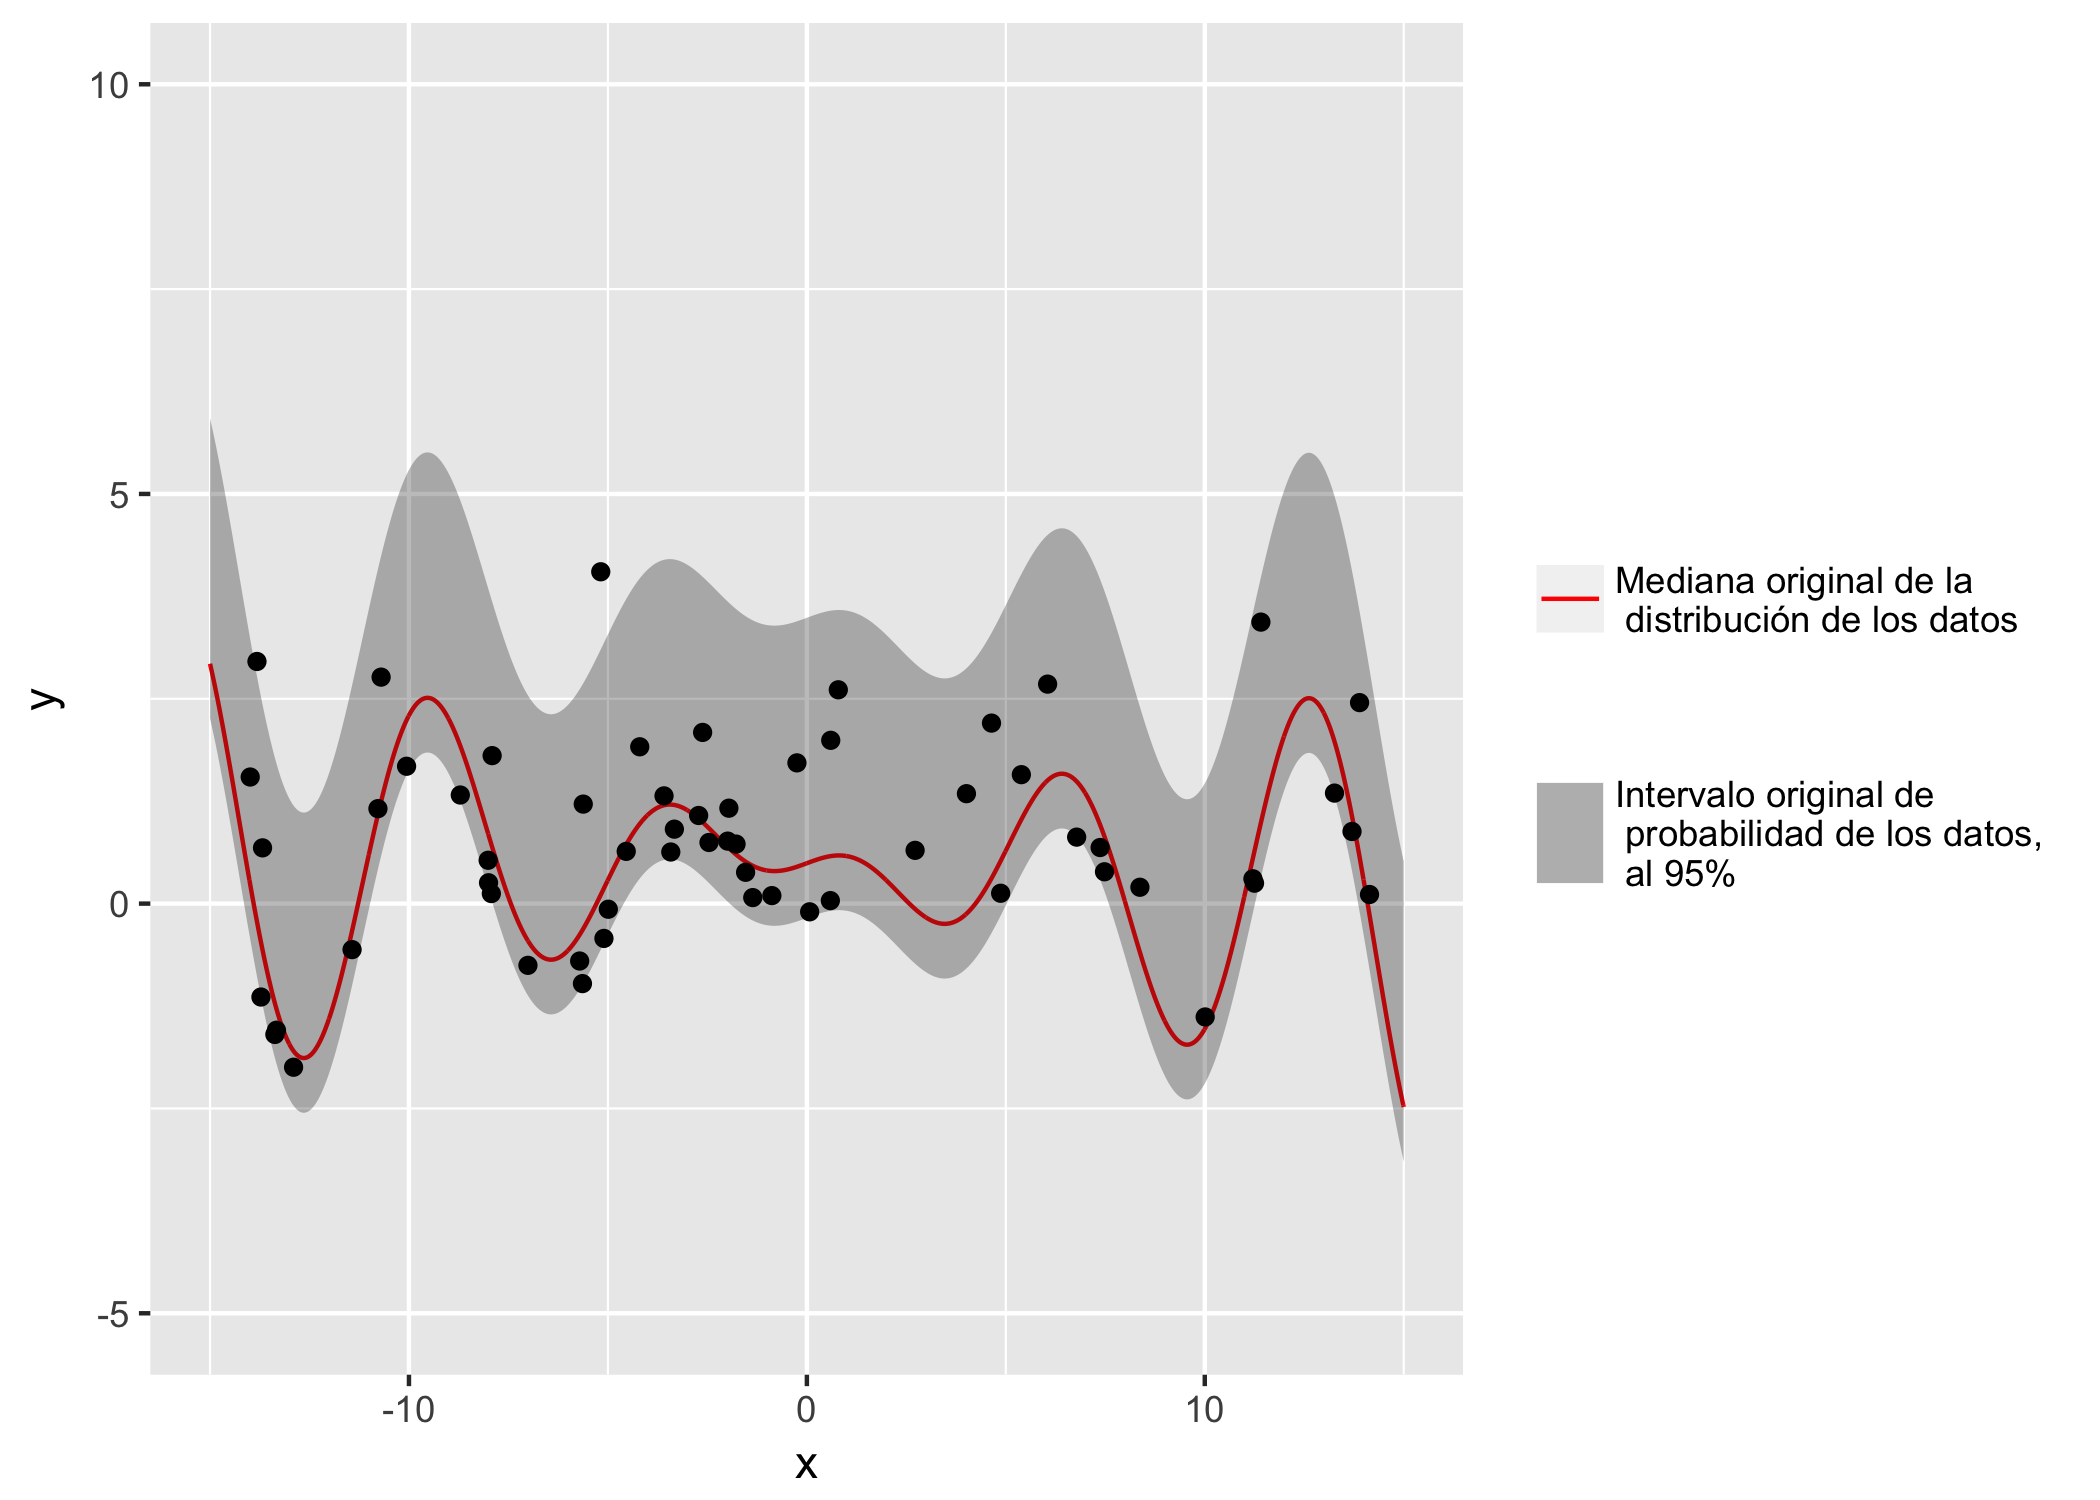
\includegraphics[width=0.7\textwidth]{Figures/Simulation/asymmetric/sample.png}
        	\label{sample_classic}
    \end{figure}
    \begin{equation*}
    \begin{aligned}
        g(x) &= \frac{1}{5} x cos(x) - \frac{1}{5}exp\left(\frac{x}{10}\right),\\
        \omega &\sim Gamma(1,1)
    \end{aligned}
    \end{equation*}
\end{frame}

\begin{frame}{Error aleatorio asim\'etrico}
    \begin{figure}[H]
        \centering
        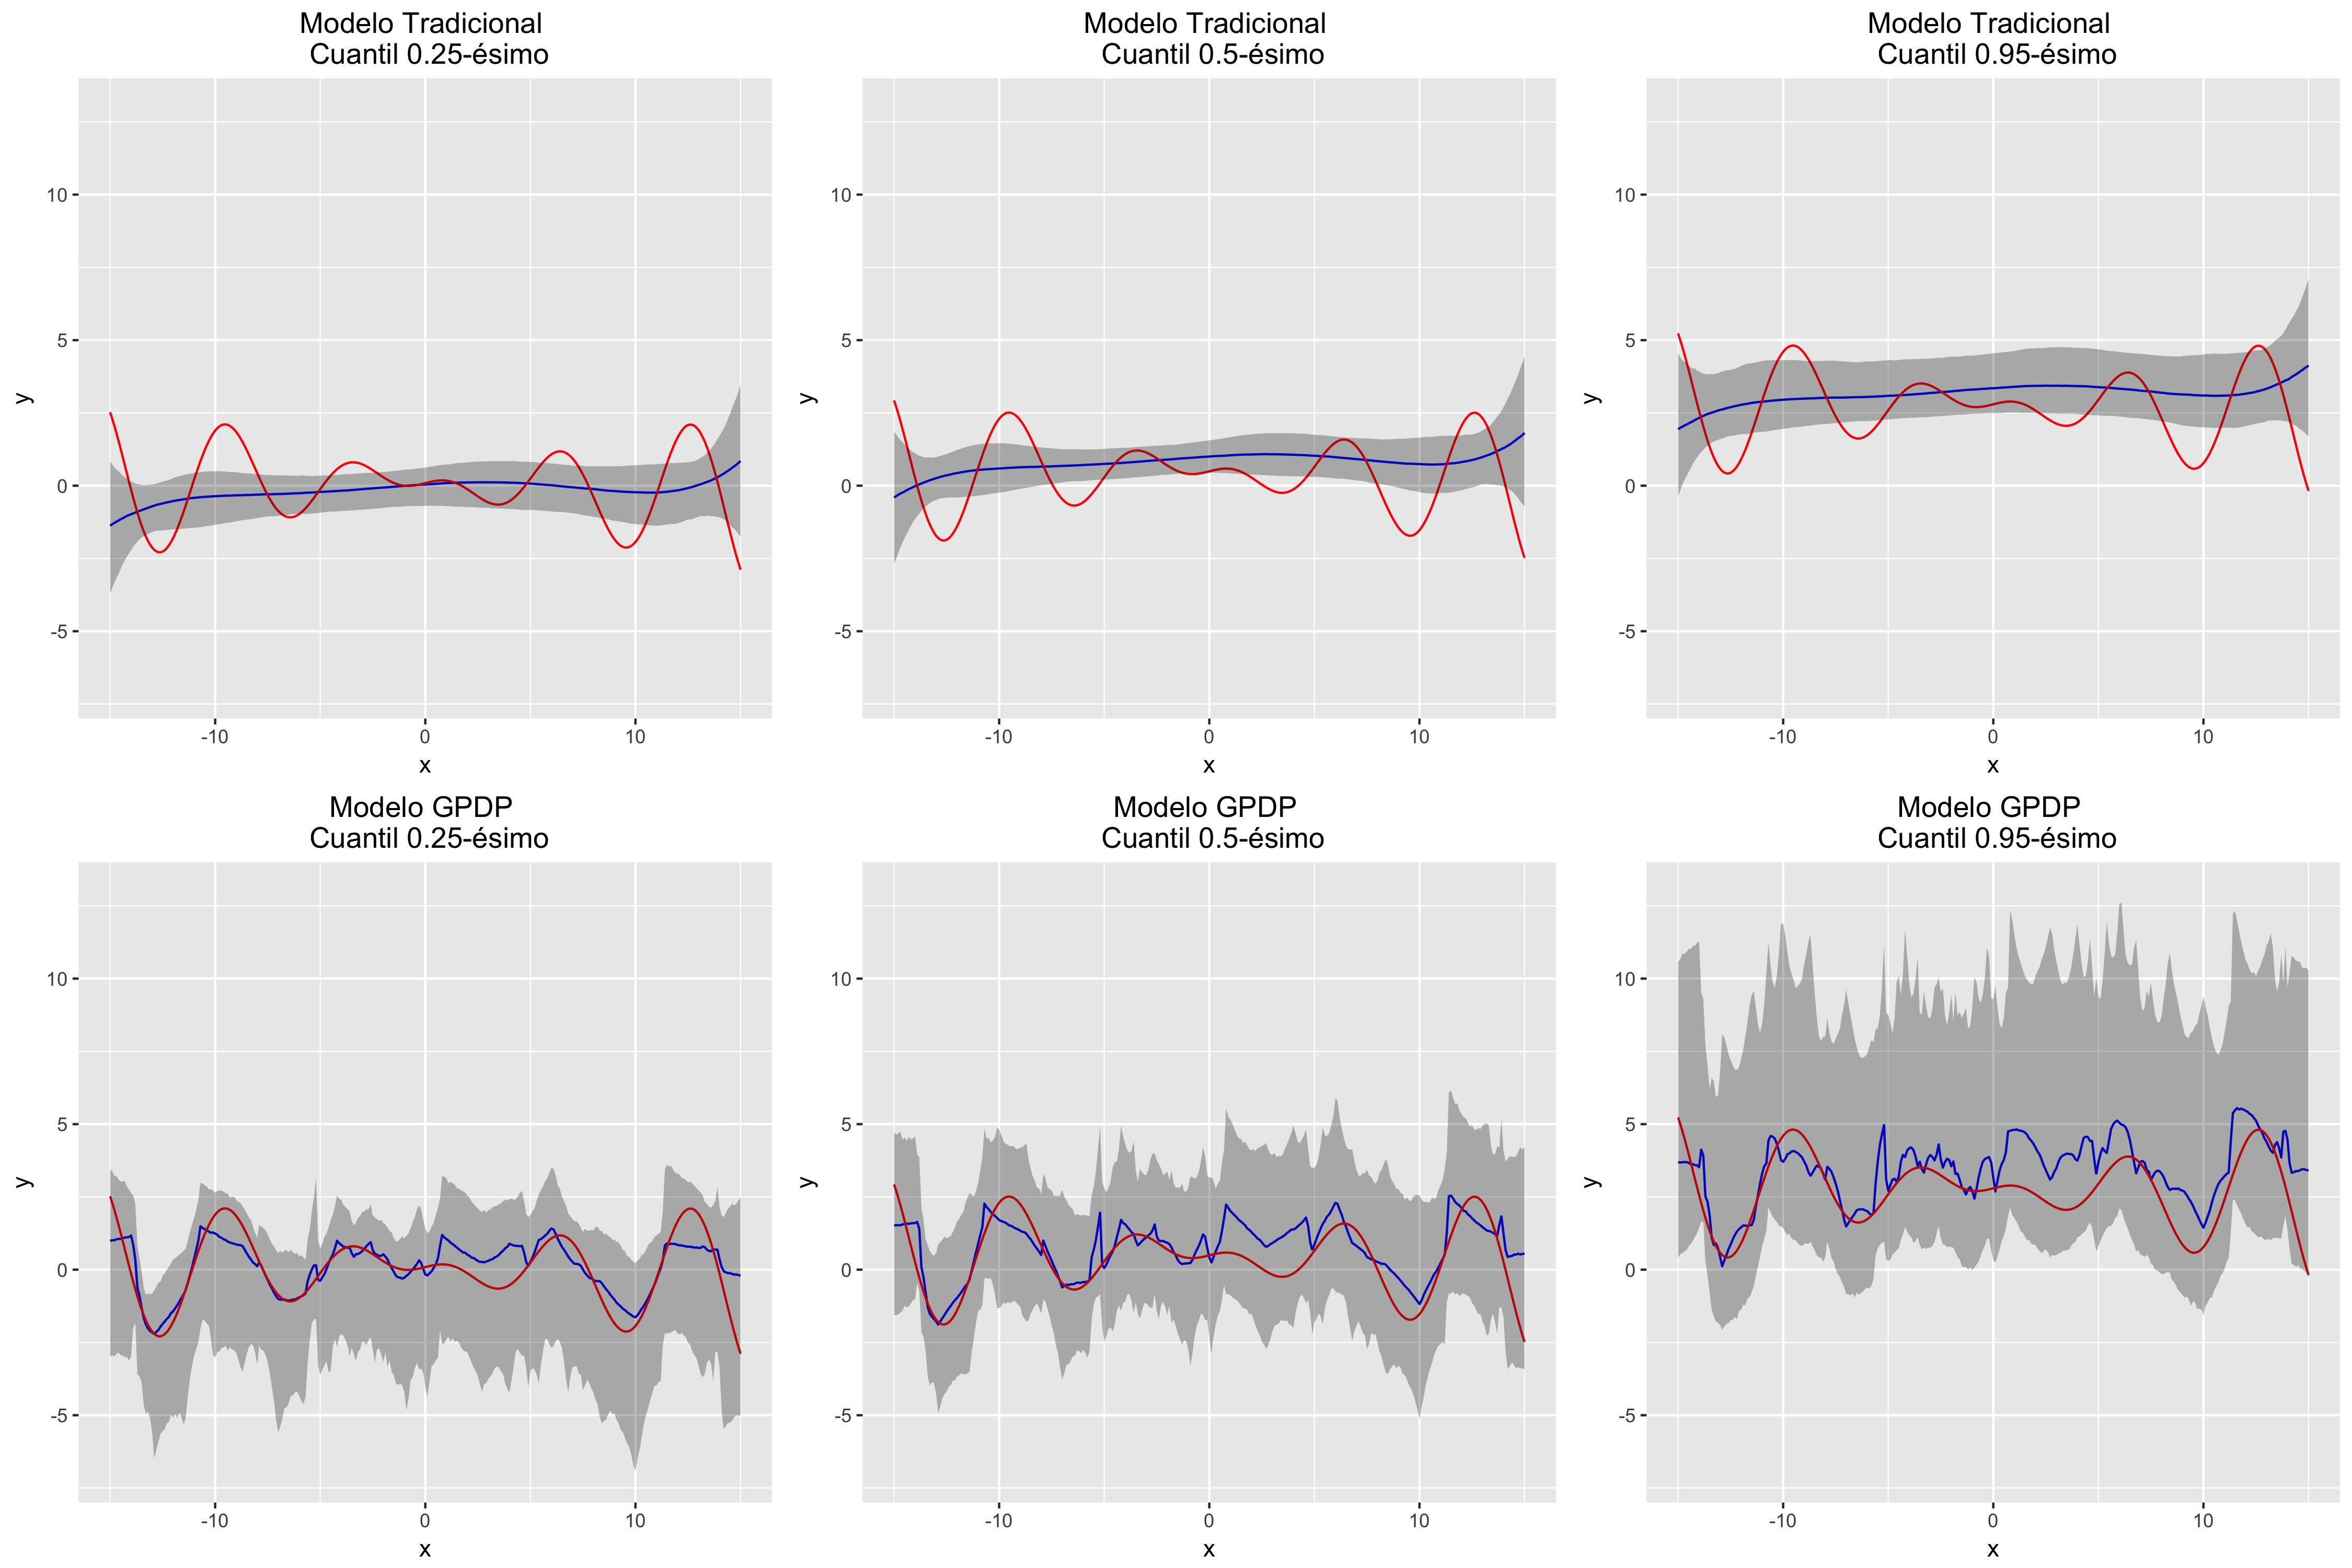
\includegraphics[width=0.8\textwidth]{Figures/Simulation/asymmetric/presentation.png}
        \captionsetup{singlelinecheck=off,font=footnotesize}
        \caption*{Nota: La l\'inea roja representa el valor real de cada cuantil, la l\'inea azul representa la mediana de la distribuci\'on posterior predictiva y el \'area gris su intervalo de probabilidad al 95\%.}
    \end{figure}
\end{frame}

\begin{frame}{Error aleatorio asim\'etrico}

\begin{scriptsize}

\begin{table}[H]
    \centering
    \caption{Error cuadr\'atico medio entre mediana predictiva y cuantil real}
    \begin{tabular}{ccc}
    \hline
    Cuantil & Modelo Tradicional & Modelo GPDP \\ 
    \hline
    0.95 & 1.69 & 1.23 \\ 
    0.50 & 1.65 & 0.64 \\ 
    0.25 & 1.53 & 0.44 \\
    \hline
    \end{tabular}
\end{table}
\begin{table}[H]
    \centering
    \caption{Correlaci\'on al cuadrado entre mediana predictiva y cuantil real} 
    \begin{tabular}{ccc}
    \hline
    Cuantil & Modelo Tradicional & Modelo GPDP \\ 
    \hline
    0.95 & 0.01 & 0.50 \\ 
    0.50 & 0.01 & 0.61 \\ 
    0.25 & 0.01 & 0.69 \\ 
    \hline
    \end{tabular}
\end{table}

\begin{table}[H]
    \centering
    \caption{Porcentaje de valores reales dentro del intervalo de confianza al 95$\%$} 
    \begin{tabular}{ccc}
    \hline
    Cuantil & Modelo Tradicional & Modelo GPDP \\ 
    \hline
    0.95 & 58\% & 100\% \\ 
    0.50 & 46\% & 100\% \\ 
    0.25 & 52\% & 100\% \\ 
    \hline
    \end{tabular}
\end{table}

\end{scriptsize}
\end{frame}

% \begin{frame}{Heterocedasticidad en el error}
%     \begin{figure}[H]
%         	\centering
%         	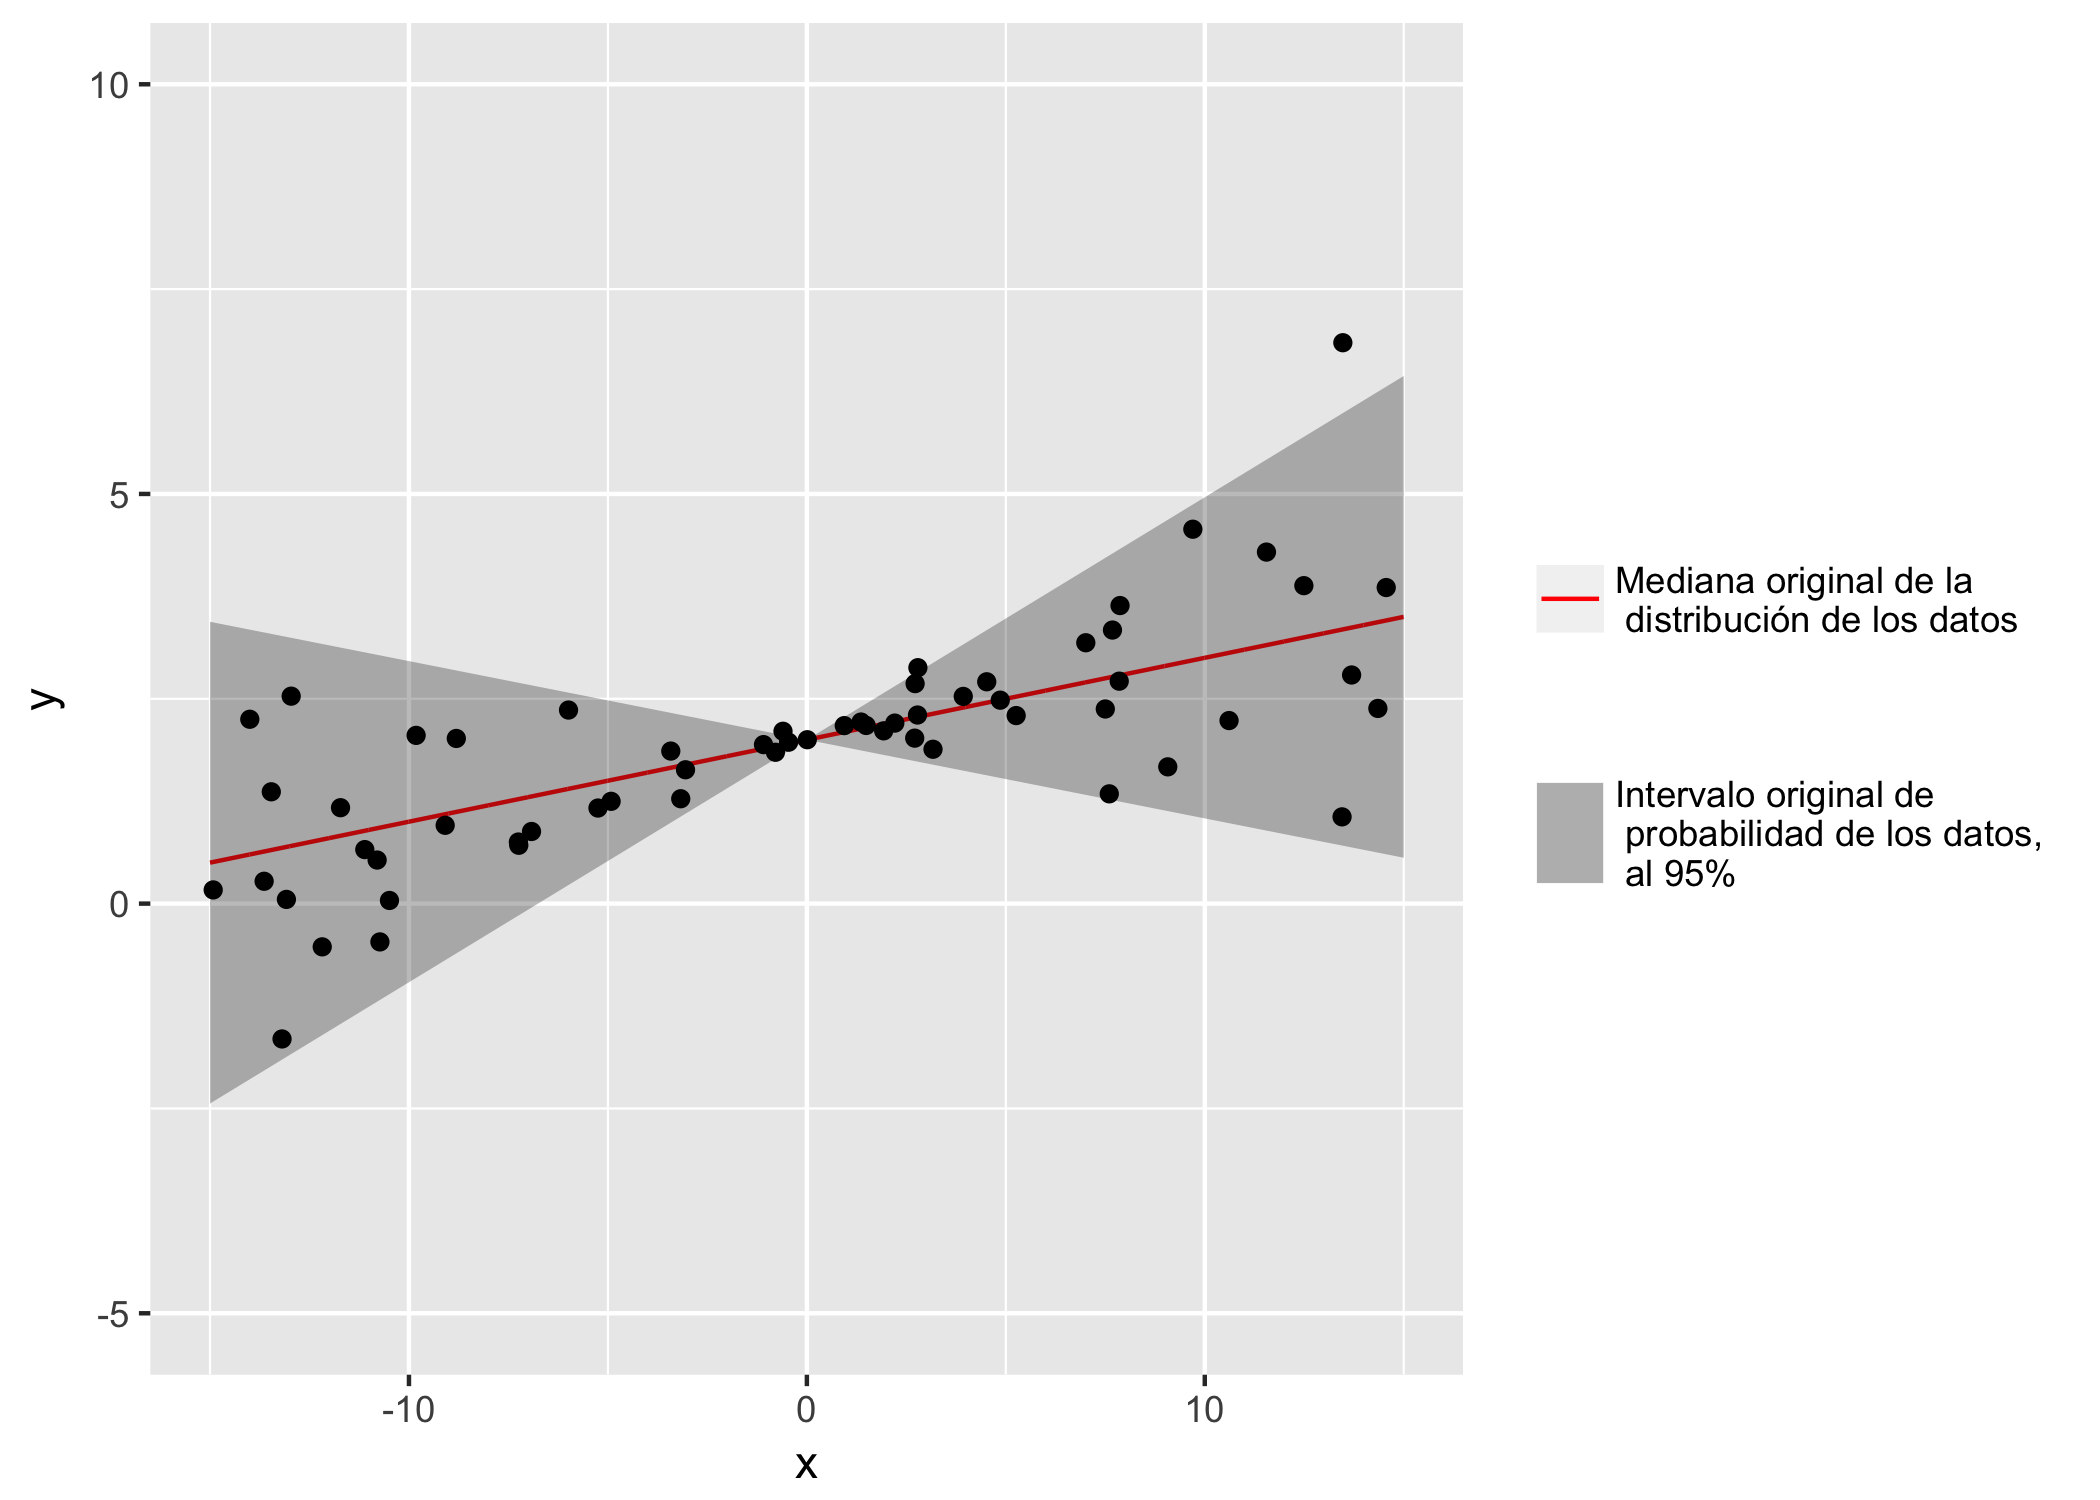
\includegraphics[width=0.65\textwidth]{Figures/Simulation/heteroscedasticity/sample.png}
%         	\label{sample_classic}
%     \end{figure}
%     \begin{equation*}
%     \begin{aligned}
%         g(x) &= \frac{1}{10}x + 2,\\
%         \omega(x) &\sim \mathcal{N}\left(0,\frac{|x|}{10}\right)
%     \end{aligned}
%     \end{equation*}
% \end{frame}

% \begin{frame}{Heterocedasticidad en el error}

% \begin{scriptsize}

% \begin{table}[H]
%     \centering
%     \caption{Error cuadr\'atico medio entre mediana predictiva y cuantil real}
%     \begin{tabular}{ccc}
%     \hline
%     Cuantil & Modelo Tradicional & Modelo GPDP \\ 
%     \hline
%     0.95 & 0.51 & 0.58 \\ 
%     0.50 & 0.02 & 0.17 \\ 
%     0.25 & 0.15 & 0.14 \\
%     \hline
%     \end{tabular}
% \end{table}
% \begin{table}[H]
%     \centering
%     \caption{Correlaci\'on al cuadrado entre mediana predictiva y cuantil real} 
%     \begin{tabular}{ccc}
%     \hline
%     Cuantil & Modelo Tradicional & Modelo GPDP \\ 
%     \hline
%     0.95 & 0.63 & 0.78 \\ 
%     0.50 & 0.98 & 0.86 \\ 
%     0.25 & 0.86 & 0.84 \\ 
%     \hline
%     \end{tabular}
% \end{table}

% \begin{table}[H]
%     \centering
%     \caption{Porcentaje de valores reales dentro del intervalo de confianza al 95$\%$} 
%     \begin{tabular}{ccc}
%     \hline
%     Cuantil & Modelo Tradicional & Modelo GPDP \\ 
%     \hline
%     0.95 & 68\% & 95\% \\ 
%     0.50 & 100\% & 100\% \\ 
%     0.25 & 81\% & 100\% \\ 
%     \hline
%     \end{tabular}
% \end{table}

% \end{scriptsize}
% \end{frame}

\begin{frame}{Comparaci\'on de tiempos}
\begin{scriptsize}
\begin{table}[H]
\centering
\caption{Tiempo de ajuste por conjunto de datos, para cada modelo.} 
\begin{tabular}{ccc}
  \hline
Datos & Tradicional (seg) & GPDP (seg) \\ 
  \hline
Supuestos tradicionales & menos de 1 & 2,498 \\ 
  Colas pesadas & menos de 1 & 4,006 \\ 
  Heterocedasticidad & menos de 1 & 3,502 \\ 
  Error asim\'etrico & menos de 1 & 6,707 \\ 
  Discontinuidades & menos de 1 & 3,062 \\ 
   \hline
\end{tabular}
\label{fit_time}
\end{table}

\begin{table}[H]
\centering
\caption{Tiempo de predicci\'on por conjunto de datos, para cada modelo.} 
\begin{tabular}{ccc}
  \hline
Datos & Tradicional (seg) & GPDP (seg) \\ 
  \hline
Supuestos tradicionales & 6 & 564 \\ 
  Colas pesadas & 5 & 529 \\ 
  Heterocedasticidad & 5 & 534 \\ 
  Error asim\'etrico & 6 & 537 \\ 
  Discontinuidades & 5 & 533 \\ 
   \hline
\end{tabular}
\label{pred_time}
\end{table}   
\end{scriptsize}
\end{frame}

\section{Conclusiones y trabajo futuro}

\begin{frame}{Conclusiones}
    \begin{itemize}
        \setlength\itemsep{2em}
        \item {Si bien los \textbf{modelos de regresi\'on a la media} han sido de mucha utilidad en las \'ultimas d\'ecadas, existen \textbf{contextos} en los que resultan \textbf{insuficientes}.}
        \item {Crear modelos que permitan una \textbf{mayor flexibilidad}, como aquellos que utilizan \textbf{m\'etodos no param\'etricos}, lograr\'a una \textbf{representaci\'on m\'as certera} de la realidad de la que provienen los datos.}
        \item {Un reto importante que present\'o este trabajo fue el \textbf{desarrollo del paquete en R}, tanto por el \textbf{planteamiento te\'orico del simulador de Gibbs}, como por la b\'usqueda de una \textbf{programaci\'on general y eficiente}.}
    \end{itemize}
\end{frame}{}

\begin{frame}{Trabajo futuro}
    \begin{itemize}
        \setlength\itemsep{2em}
        \item {Proponer alguna manera de darle un \textbf{peso distinto a cada variable explicativa}, en el proceso Gaussiano. Actualmente toma una \'unica distancia, dando igual peso a cada variable.}
        \item {Ser\'ia conveniente la inclusi\'on de un \textbf{par\'ametro de rango} que regule din\'amicamente la relaci\'on entre la \textbf{distancia y la covarianza} entre observaciones, en el proceso Gaussiano.}
        \item {Desarrollar una medida robusta de \textbf{bondad de ajuste}, que permita hacer selecci\'on de variables y comparaci\'on con otros modelos disponibles). }
        
    \end{itemize}
\end{frame}

\begin{frame}
  \titlepage
\end{frame}

\end{document}


